\section{Práticas sugeridas pela \playAPC} \label{sec:praticas}
Baseado nos tópicos mais recorrentes da matéria inicial dos cursos de computação, explicado na Seção \ref{sec:projeto}, foram feitos 24 exercícios no total, separados por tópicos. Todos os exercícios, juntamente com sua solução e comentários, podem ser consultados na apostila de exercício (Apêndice \ref{appendix:apostila}). Nesta aposila, ainda são encontrado mais 3 exercícios extras, que abordam todos os tópicos juntos.

Para melhor visualização, os códigos-fontes de todos os exercícios propostos nesta Seção também podem ser encontrados no Apêndice \ref{appendix:src}.
\subsection{Tipo de dados e estruturas de controle}

\begin{renumerate}
 \item) Exiba um plano cartesiano de -100 a 100 com espaçamento de 5 unidades.
  \label{ex:cap01_ex1}

  \begin{figure}[H]
    \centering
    \begin{subfigure}[t]{0.2\textwidth}
        \centerline{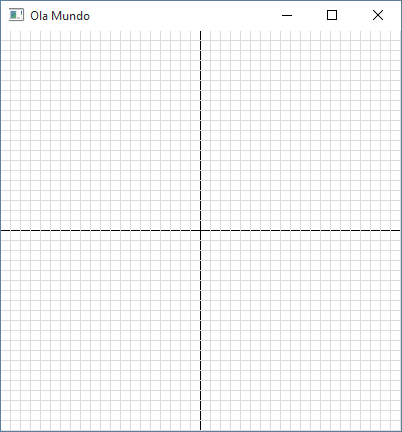
\includegraphics[width=.9\textwidth]{img/cap1_ex1.png}}
        \caption{Visualização de todo plano cartesiano.}
        \label{fig:cap01_ex1}
    \end{subfigure}
    ~
    \begin{subfigure}[t]{0.65\textwidth}
        \centerline{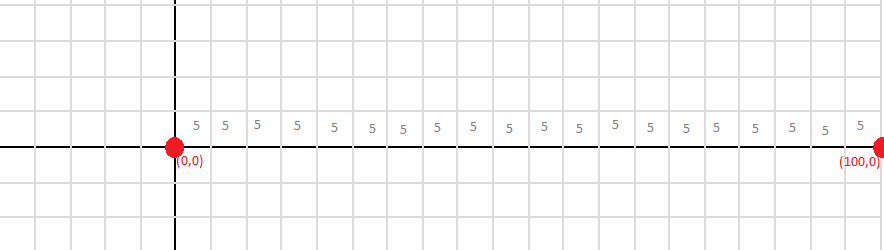
\includegraphics[width=.9\textwidth]{img/cap1_ex1_b.png}}
        \caption{De (0,0) até (100,0), existem 20 quadrados com 5 unidades de tamanho.}
        \label{fig:cap01_ex1}
    \end{subfigure}
    \caption{Plano cartesiano de -100 à 100: a) Todo plano; b) Parte do plano.}
\end{figure}


 Comentário: Esta prática se refere a exibir um Plano Cartesiano na tela com espaçamento de 5 em 5 unidades, tanto no eixo x quanto no eixo y. Com ela, o aluno poderá notar a importância da ordem de chamada de funções da \playAPC{} e a necessidade das funções \emph{AbreJanela} e \emph{Desenha}, além de verificar, com um exemplo simples, se a playAPC{} foi corretamente instalada.

%\lstinputlisting[caption=Código fonte de Plano Cartesiano, style=code, label=lst:cap1_ex1]{src/ex1_PrimeiraJanela.cpp}


\item) \label{ex:cap01_ex2} Exiba um boneco palito.
  
  \begin{figure}[H]
    \centerline{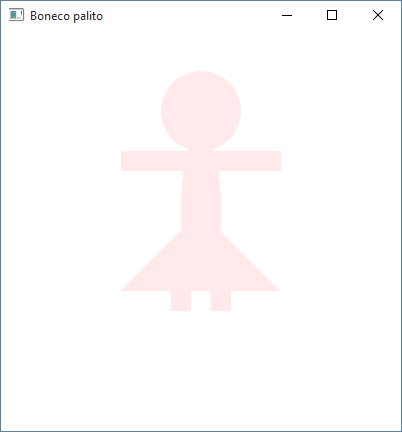
\includegraphics[width=.25\textwidth]{img/cap1_ex3.png}}
    \caption{Boneco Palito.}
    \label{fig:cap01_ex2}
  \end{figure}

 Comentário: Esta prática se refere a exibir um boneco palito e praticar a grande maioria das geometrias pré-definidas existentes na \playAPC{}. Os argumentos de cada função podem ser consultados no Guia de Referência da \playAPC \footnote{\url{http://playapc.zaghetto.com/category/funcoes/geometrias}}.
%\lstinputlisting[caption=Código fonte do boneco palito, style=code, label=lst:cap1_ex2]{src/ex3_boneco.cpp}

\item)
 Exiba a estrela de Davi.
  \label{ex:cap01_ex3}

  \begin{figure}[H]
    \centerline{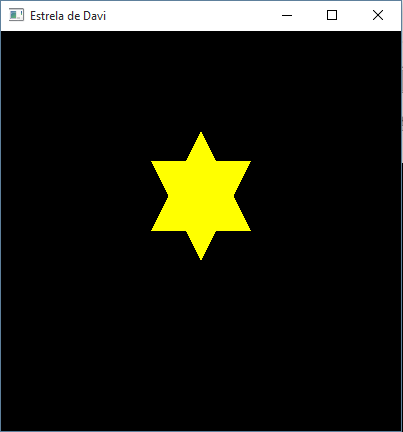
\includegraphics[width=.25\textwidth]{img/cap1_ex2.png}}
    \caption{Estrela de Davi.}
    \label{fig:cap01_ex3}
  \end{figure}

  Comentário: Esta prática se refere a exibir a estrela de Davi, feita com dois triângulos. Um triângulo foi criado com a função \emph{CriaTriangulo} e o outro com a função \emph{CriaPoligono}. Verificamos nesta prática os argumentos de \emph{CriaTriangulo} (base, altura e ponto esquerdo inferior) e, como não há como ter altura negativa, teve a necessidade de criar um polígono definido pelos três pontos \emph{p1, p2} e \emph{p3} para criar-se um triângulo \emph{de cabeça pra baixo}.
%\lstinputlisting[caption=Código fonte da Estrela de Davi, style=code, label=lst:cap1_ex3]{src/ex2_davi.cpp}

  \item)
  Escreva um programa que solicite do usuário um raio de um círculo e exiba um quadrado inscrito neste círculo.
  \label{ex:cap01_ex8}

  \begin{figure}[H]
    \centerline{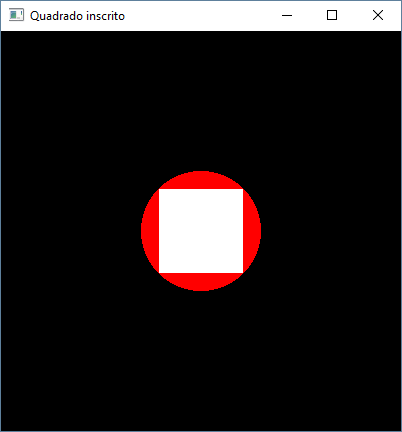
\includegraphics[width=.3\textwidth]{img/cap1_ex21}}
    \caption{Quadrado inscrito em um círculo.}
    \label{fig:cap01_ex8}
  \end{figure}

  Comentário: Esta prática se refere a exibir um quadrado inscrito em um círculo, a qual exercita o raciocínio matemático do aluno. O quadrado, criado pela função \emph{CriaQuadrado}, precisa de um ponto de referência para ser criado, sendo este ponto o inferior esquerdo. Desta forma, o aluno teria que calcular, dado o raio do círculo, não apenas o lado do quadrado, mas também a posição que este ponto de referência precisa estar.

%\lstinputlisting[caption=Código fonte do quadrado inscrito, style=code, label=lst:cap1_ex8]{src/ex21_inscrito.cpp}


  \item)
  Escreva um programa que solicita do usuário um raio, a posição do centro de uma circunferência e a posição de um ponto qualquer. Exiba a cena e indique no título da janela se o ponto está dentro ou fora da circunferência.

   \begin{figure*}[!htb]
    \centering
    \begin{subfigure}[t]{0.3\textwidth}
        \centerline{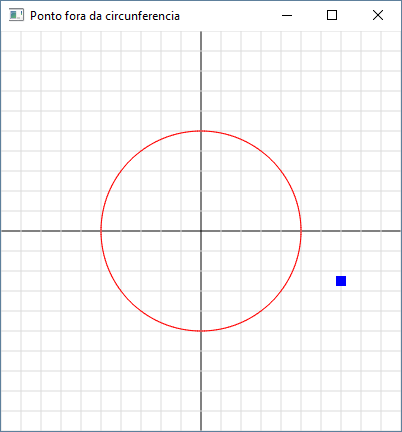
\includegraphics[width=.9\textwidth]{img/cap1_ex22}}
        \caption{Ponto está fora da circunferência.}
        \label{fig:cap01_ex22a}
    \end{subfigure}
    ~
    \begin{subfigure}[t]{0.3\textwidth}
        \centerline{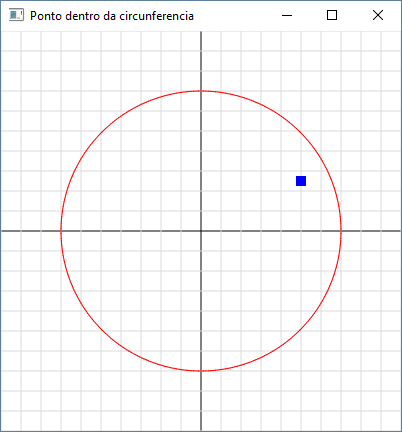
\includegraphics[width=.9\textwidth]{img/cap1_ex22b}}
        \caption{Ponto está dentro da circunferência.}
        \label{fig:cap01_ex22b}
    \end{subfigure}
    \caption{Verificação se ponto está dentro ou fora da circunferência: a) Fora; b) Dentro.}
  \end{figure*}

  \label{ex:cap01_ex22}

  Comentário: Esta prática exibe uma circunferência e indica se dado um ponto qualquer, se este ponto está dentro ou fora da circunferência, exercitando o conceito de distância entre dois pontos. Para a ampliação da espessura do ponto, para ele não ser apenas um pixel, utiliza-se a função \emph{Grafite}.

%\lstinputlisting[caption=Código fonte do ponto dentro ou fora da circunferência, style=code, label=lst:cap1_ex22]{src/ex22_inout.cpp}

\item)
Escreva um programa que receba do usuário um valor de ângulo em graus e um valor de raio. Converta para radianos o ângulo e exiba uma reta com o raio fornecido pelo usuário e pinte-a de acordo com as seguintes regras:
    \begin{itemize}
    \item
    Se a reta pertencer ao \emph{primeiro} quadrante, pinte-a de vermelho
    \item
    Se a reta pertencer ao \emph{segundo} quadrante, pinte-a de verde
    \item
    Se a reta pertencer ao \emph{terceiro} quadrante, pinte-a de azul
    \item
    Se a reta pertencer ao \emph{quarto} quadrante, pinte-a de preto
    \end{itemize}
    \label{ex:cap01_ex4}

  \begin{figure*}[h!]
    \centering
    \begin{subfigure}[t]{0.2\textwidth}
        \centerline{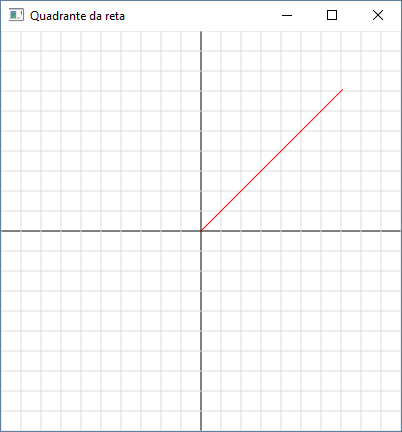
\includegraphics[width=.9\textwidth]{img/cap1_ex4}}
        \caption{Reta pertencente ao primeiro quadrante.}
        \label{fig:cap01_ex4a}
    \end{subfigure}
    ~
    \begin{subfigure}[t]{0.2\textwidth}
        \centerline{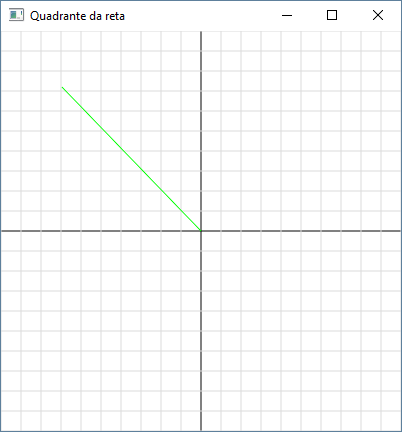
\includegraphics[width=.9\textwidth]{img/cap1_ex4b}}
        \caption{Reta pertencente ao segundo quadrante.}
        \label{fig:cap01_ex4b}
    \end{subfigure}
    ~
    \begin{subfigure}[t]{0.2\textwidth}
        \centerline{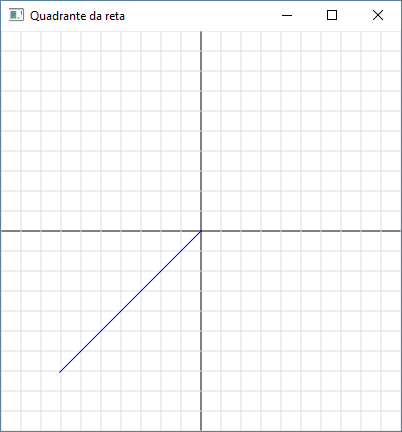
\includegraphics[width=.9\textwidth]{img/cap1_ex4c}}
        \caption{Reta pertencente ao terceiro quadrante.}
        \label{fig:cap01_ex4c}
    \end{subfigure}
    ~
    \begin{subfigure}[t]{0.2\textwidth}
        \centerline{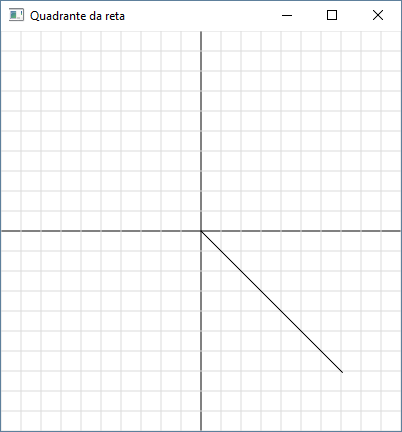
\includegraphics[width=.9\textwidth]{img/cap1_ex4d}}
        \caption{Reta pertencente ao quarto quadrante.}
        \label{fig:cap01_ex4d}
    \end{subfigure}
    \caption{Identificação de quadrante: a) Primeiro quadrante; b) Segundo quadrante; c) Terceiro quadrade; d) Quarto quadrante.}
\end{figure*}

  Comentário: Esta prática exibe uma reta com cor variada de acordo com qual quadrante ela pertence. A função \emph{Pintar} neste caso se refere a única geometria criada no programa, no caso, a reta.
%\lstinputlisting[caption=Código fonte do quadrante da reta, style=code, label=lst:cap1_ex4]{src/ex4_reta.cpp}

\item)
Escreva um programa em C que solicita três pontos A, B e C ao usuário, e verifica se esses valores satisfazem a condição de existência do triângulo. Caso essa condição seja satisfeita, exiba esse triângulo e escreva no título da janela se o triângulo é equilátero, isósceles ou escaleno [dica: não usar a função CriaTriangulo()].

  \begin{figure}[H]
    \centering
    \begin{subfigure}[t]{0.3\textwidth}
        \centerline{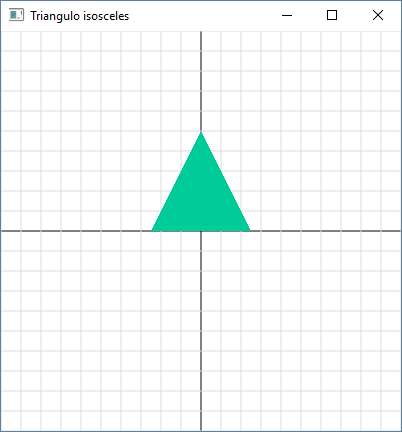
\includegraphics[width=.9\textwidth]{img/cap1_ex23}}
        \caption{Triângulo isósceles.}
        \label{fig:cap01_ex23a}
    \end{subfigure}
    ~
    \begin{subfigure}[t]{0.3\textwidth}
        \centerline{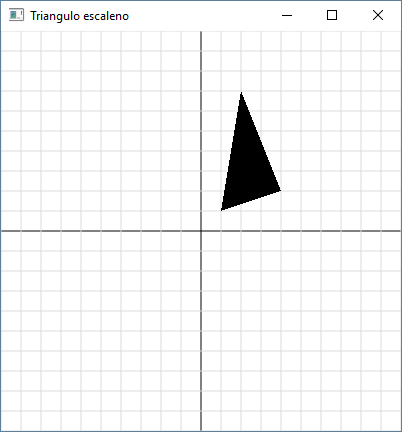
\includegraphics[width=.9\textwidth]{img/cap1_ex23b}}
        \caption{Triângulo escaleno.}
        \label{fig:cap01_ex23b}
    \end{subfigure}
    ~
    \begin{subfigure}[t]{0.3\textwidth}
        \centerline{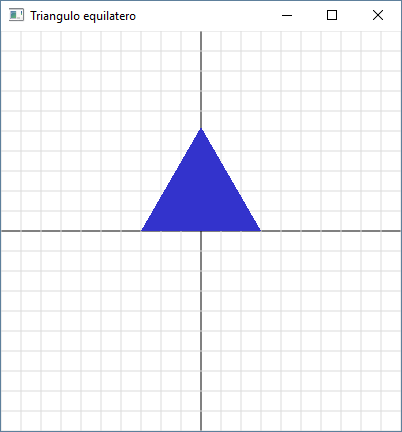
\includegraphics[width=.9\textwidth]{img/cap1_ex23c}}
        \caption{Triângulo equilátero.}
        \label{fig:cap01_ex23c}
    \end{subfigure}
    \caption{Existência de triângulos: a) Isósceles; b) Escaleno; c) Equilátero.}
\end{figure}

\label{ex:cap01_ex23}

Comentário: Esta prática exercita o conceito matemático de condição de existência e de classificação de triângulo, além de exercitar \emph{ifs} aninhados.

%\lstinputlisting[caption=Código fonte de exibir triângulo caso ele exista, style=code, label=lst:cap1_ex23]{src/ex23_exibetriangulo.cpp}


\item)
Exiba um carrinho se movendo de $-100$ à $100$.
  \label{ex:cap01_ex6}

  \begin{figure}[H]
    \centerline{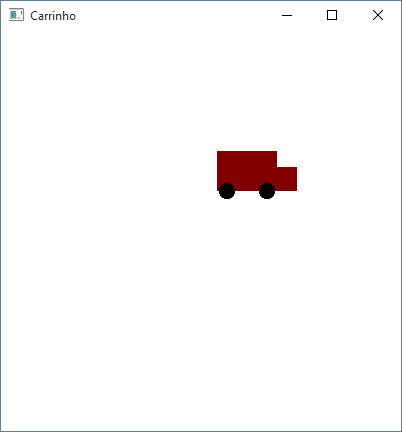
\includegraphics[width=.3\textwidth]{img/cap1_ex5.png}}
    \caption{Carro se movendo da posição -100 até a posição 100.}
    \label{fig:cap01_ex6}
  \end{figure}

 Comentário: Esta prática exibe um carro construído com dois retângulos e dois círculos, agrupados com a função \emph{CriaGrupo}, movendo-se da posição -100 até a posição 100. Nota-se que todas as geometrias que estão abaixo da função \emph{CriaGrupo} pertencem a um único grupo, o grupo \emph{carro}.
%\lstinputlisting[caption=Código fonte do carro andando, style=code, label=lst:cap1_ex6]{src/ex5_carrinho.cpp}

\item)
Construa um moinho de vento e coloque apenas as hélices para girar.
  \label{ex:cap01_ex7}

  \begin{figure}[H]
    \centerline{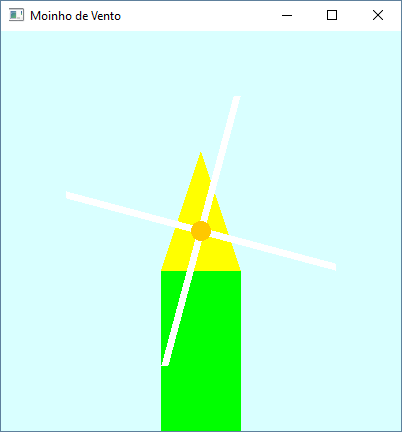
\includegraphics[width=.3\textwidth]{img/cap1_ex7.png}}
    \caption{Moinho de vento.}
    \label{fig:cap01_ex7}
  \end{figure}

  Comentário: Esta prática exibe um moinho de vento criado com um grupo composto por um triângulo e um retângulo, o grupo \emph{moinho}, e outro grupo composto pelas hélices, o grupo \emph{helices}. Somente o \emph{helices} sofre a ação de girar. 
%\lstinputlisting[caption=Código fonte do moinho, style=code, label=lst:cap1_ex7]{src/ex7_moinho.cpp}

\item)
Escreva um programa utilizando a playAPC que simule simultaneamente o movimento da Terra ao redor do Sol e o movimento da Lua ao redor da Terra. Considere que as trajetórias de ambas são elípticas. No caso da Terra, o Sol é um dos focos e no caso da Lua, a Terra é um dos focos. Não é necessário simular a proporção real entre os semieixos maiores (a) da Lua e da Terra, nem a excentricidade (e) das duas trajetórias. Encontre empiricamente valores de (a) e (e) de forma que seja possível observar trajetórias elípticas. Simule, porém, a proporção real entre os movimento de translação da Terra e da Lua.
  \label{ex:cap01_ex24}

  \begin{figure}[H]
    \centerline{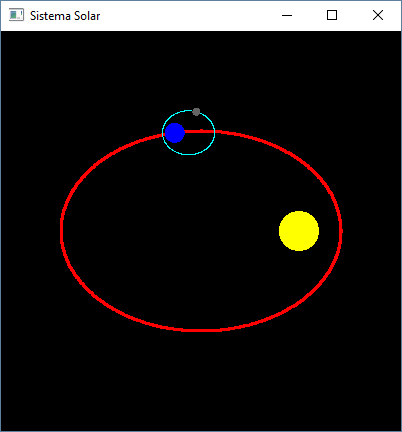
\includegraphics[width=.3\textwidth]{img/cap1_ex24.png}}
    \caption{Sistema solar.}
    \label{fig:cap01_ex24}
  \end{figure}

  Comentário: Esta prática ilustra, de maneira exagerada, o movimento elíptico de um sistema solar, reforçando que a lua deve girar em torno da terra de maneira mais rápida que a terra deve girar ao redor da lua.
%\lstinputlisting[caption=Código fonte do sistema solar, style=code, label=lst:cap1_ex24]{src/ex24_solar.cpp}

\item)
Sabe-se que a equação da espiral hiperbólica pode ser defina por
\begin{equation} \label{eq:espiral}
  \begin{matrix}
  x & = & a \cos(\theta) \\ 
  y & = & a \sin(\theta)
  \end{matrix}.
\end{equation}
  onde $a$ é a assíntota para y e $\theta$ o ângulo equivalente ao ângulo em coordenadas polares. Para $a \gets 100$ e $\theta \in (0, 4\pi)$, desenhe duas espirais hiperbólicas calculando seus pontos como é descrito na Equação \ref{eq:espiral}. Para ponto $p$ em $(x,y)$ de uma das hiperbólica, o ponto $p$ da outra espiral deve estar posicionado em $(-x,-y)$.

  \label{ex:cap01_ex5}

  \begin{figure*}[!htp]
    \centering
    \begin{subfigure}[t]{0.3\textwidth}
        \centerline{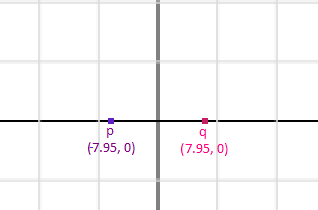
\includegraphics[width=.9\textwidth]{img/cap1_ex6}}
        \caption{Posição inicial aproximada de ambas as espirais.}
        \label{fig:cap01_ex6a}
    \end{subfigure}
    ~
    \begin{subfigure}[t]{0.3\textwidth}
        \centerline{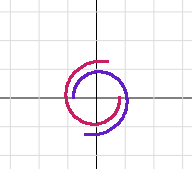
\includegraphics[width=.9\textwidth]{img/cap1_ex6b}}
        \caption{100º iteração no processo de criação das espirais.}
        \label{fig:cap01_ex6b}
    \end{subfigure}
    ~
    \begin{subfigure}[t]{0.3\textwidth}
        \centerline{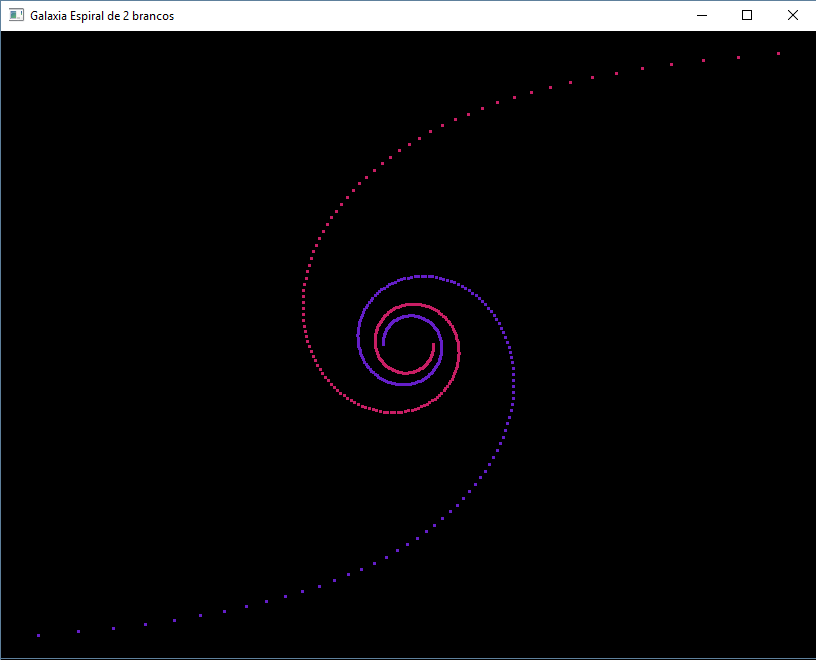
\includegraphics[width=.9\textwidth]{img/cap1_ex6c}}
        \caption{Espirais completas.}
        \label{fig:cap01_ex6c}
    \end{subfigure}
    \caption{Espiral hiperbólica: a) Primeira iteração; b) Centésima iteração; c) Espirais.}

\end{figure*}
  Comentário: Esta prática ilustra como a função \emph{Desenha1Frame} pode ser utilizada. 
%\lstinputlisting[caption=Código fonte da galáxia expiral, style=code, label=lst:cap1_ex5]{src/ex6_galaxy.cpp}


  \item)
  Crie uma animação em que o Mário deve começar no canto esquerdo da tela e seu objetivo é andar até o canto direito da tela. Porém, haverão dois canos que serão posicionados aleatoriamente no meio do caminho, forçando o Mário a pulá-los para não colidir com eles. 
  Para criar a animação de andar, altere as imagens do retângulo onde será desenhado o Mario com a função \emph{AssociaImagem} e, após essa chamada, utilize a função \emph{Desenha1Frame} para renderizar a troca de imagens.

  Para simplificação do problema, considere que o Mário, ao realizar o pulo, ele deva executar meia trajetória circular, onde $\theta$ varia de $\pi$ até $0$ e o raio do pulo seja de $40$ unidades.
  \label{ex:cap01_ex25}

  \begin{figure}[H]
    \centering
    \begin{subfigure}[t]{0.3\textwidth}
        \centerline{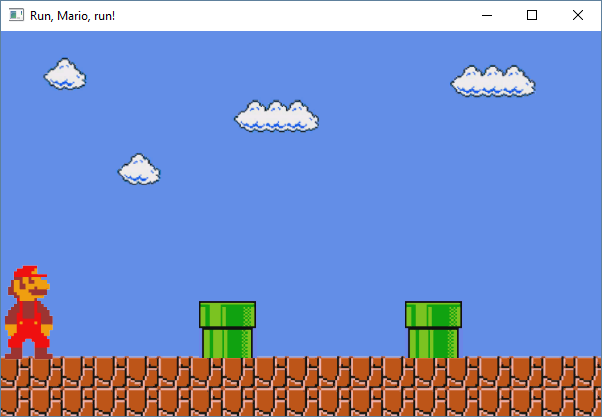
\includegraphics[width=.9\textwidth]{img/cap1_ex25}}
        \caption{Começo da animação.}
        \label{fig:cap01_ex6a}
    \end{subfigure}
    ~
    \begin{subfigure}[t]{0.3\textwidth}
        \centerline{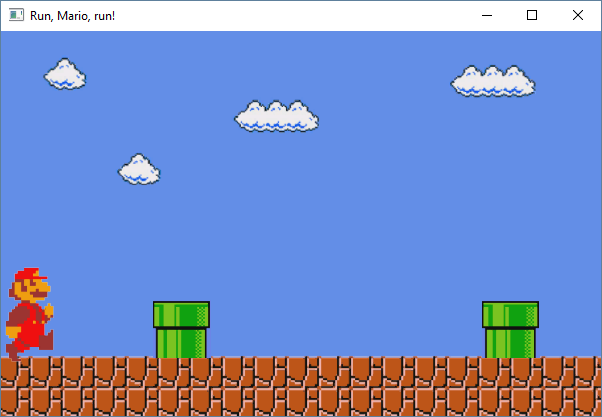
\includegraphics[width=.9\textwidth]{img/cap1_ex25b}}
        \caption{Parte 1 da animação do Mário.}
        \label{fig:cap01_ex6b}
    \end{subfigure}
    ~
    \begin{subfigure}[t]{0.3\textwidth}
        \centerline{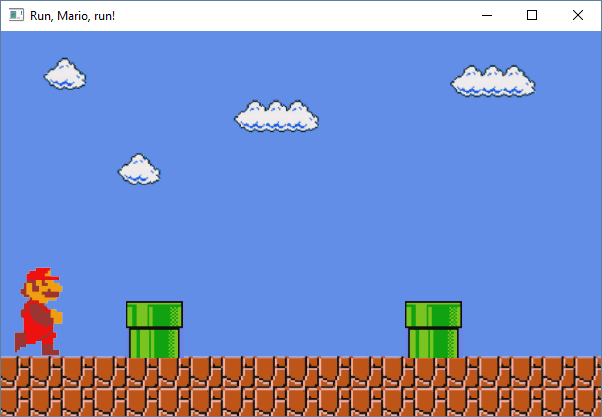
\includegraphics[width=.9\textwidth]{img/cap1_ex25c}}
        \caption{Parte 2 da animação do Mário.}
        \label{fig:cap01_ex6c}
    \end{subfigure}
    ~
    \begin{subfigure}[t]{0.3\textwidth}
        \centerline{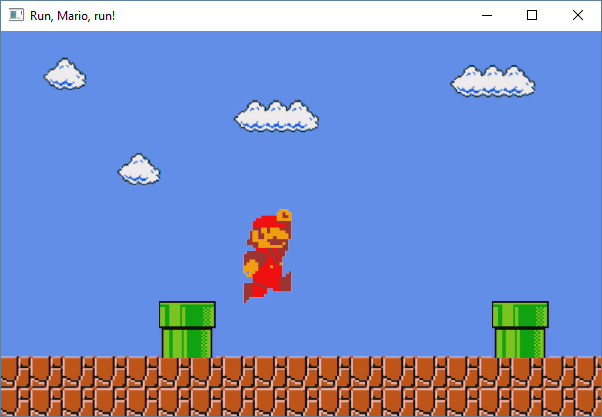
\includegraphics[width=.9\textwidth]{img/cap1_ex25d}}
        \caption{Mário pulando.}
        \label{fig:cap01_ex6c}
    \end{subfigure}
    \caption{Animação do Mário: a) Início; b) e c) Mário andando; d) Mário pulando.}
  \end{figure}

  Comentário: Esta prática introduz o conceito de colisão de objetos, com uma colisão entre dois retângulos, e também ao uso de imagens. Na introdução a utilização de imagens, não é necessário que o aluno tenha como pré-requisito o conceito de manipulação de arquivos em C. Como a função \emph{Desenha1Frame} renderiza $\frac{1}{60}$ segundos, para criar o efeito de uma animação menos fluída, se faz necessário sua chamada repetidas vezes.

%\lstinputlisting[caption=Código fonte do Mario animado, style=code, label=lst:cap1_ex25]{src/ex25_mario.cpp}

\end{renumerate}

\subsection{Vetores e Matrizes}

\begin{renumerate}
\item)
Exiba o gráfico do polinômio $-x^3$ para $-50 \leq x \leq 50$.
  \label{ex:cap02_ex1}

  \begin{figure}[ht]
    \centerline{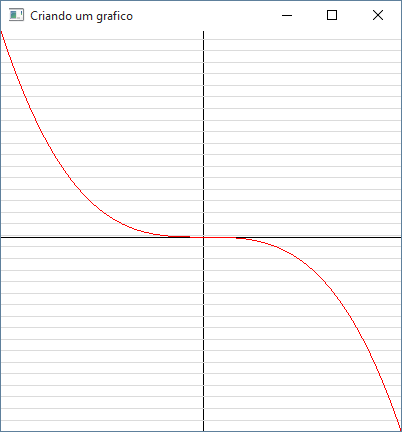
\includegraphics[width=.3\textwidth]{img/cap2_ex8.png}}
    \caption{Gráfico do polinômio $-x^3$.}
    \label{fig:cap02_ex1}
  \end{figure}

Comentário: Esta prática mostra como construir um gráfico a partir de um vetor de Pontos. Cada posição em \emph{y} de cada ponto é calculada dentro do loop. Por padrão, os limites da janela de exibição da \playAPC{} vão de -100 à 100, entretanto, os valores em \emph{y} nesta função variam de $-125.000$ até $125.000$, tendo a necessidade de mudar o limite de exibição com a função \emph{MudaLimitesJanela(125000)}.
%\lstinputlisting[caption=Código fonte do polinômio, style=code, label=lst:cap2_ex1]{src/ex8_grafico.cpp}

\item)
Escreva uma programa que solicita ao usuário 20 componentes RGB do tipo int entre 0 e 255 que são armazenadas em três vetores R, G e B. Em seguida, os valores de cada vetor são filtrados por meio da filtragem de média móvel central, como indica a Equação \ref{eq:filtro} e o resultado é armazenado em três novos vetores Rf, Gf, Bf. O tamanho da janela de filtragem é fixo e igual a 3. 

  \label{ex:cap02_ex26}

\begin{equation} \label{eq:filtro}
\begin{matrix}
Rf[i] = & \frac{R[i-1] + R[i] + R[i+1]}{3}\\ 
Gf[i] = & \frac{G[i-1] + G[i] + G[i+1]}{3}\\ 
Bf[i] = & \frac{B[i-1] + B[i] + B[i+1]}{3}
\end{matrix}
\end{equation}
\equationset{Filtragem dos componentes \emph{RGB} do componente \emph{i} com janela de filtragem igual a 3}

  Exiba graficamente dois vetores coloridos, um composto pelas componentes RGB originais e outro pelas componentes RfGfBf filtradas. No final, o programa deve calcular também a distância euclidiana média entre os dois vetores RGB e RfGfBf, como indica a Equação \ref{eq:distancia}.

  \begin{equation} \label{eq:distancia}
  \frac{1}{n}\sum_{i = 0}^{n}\sqrt{(R[i] - Rf[i])^{2} + (G[i] - Gf[i])^{2} + (B[i] - Bf[i])^{2}}
\end{equation}
\equationset{Cálculo da distância euclidiana média}

\begin{figure}[H]
    \centerline{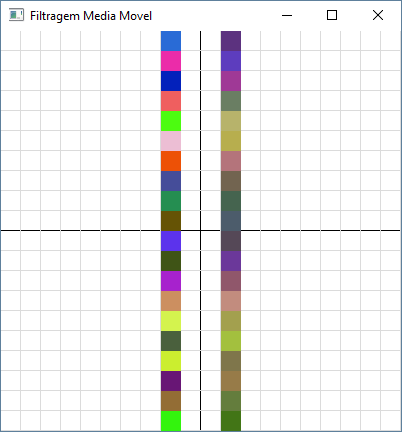
\includegraphics[width=.3\textwidth]{img/cap2_ex26.png}}
    \caption{À esquerda, 20 quadrados com componentes RGB fornecidos pelo usuário. À direita, aplicação do filtro de média móvel central em cada quadrado.}
    \label{fig:cap02_ex26}
  \end{figure}

Comentário: Esta prática exercita conceitos de processamento de imagens, aplicando um filtro dado os componentes RGB da figura, além de exercitar conceitos teóricos de matemática, como o funcionando do operador $\Sigma$.

%\lstinputlisting[caption=Código fonte do filtro de média móvel central, style=code, label=lst:cap2_ex26]{src/ex26_rgb.cpp}

\item)
O jogo da vida é um autômato celular que simula a alteração e mudanças de grupos de seres vivos. Foi criado pelo matemático John Horton Conway na década de 70. Extremamente útil para diversas áreas da ciência, este autômato possui quatro regras simples:
  \begin{enumerate}
    \item Qualquer célula viva com menos de dois vizinhos vivos morre de solidão
    \item Qualquer célula viva com mais de três vizinhos vivos morre de superpopulação
    \item Qualquer célula morta com exatamente três vizinhos vivos se torna uma célula viva
    \item Qualquer célula viva com dois ou três vizinhos vivos continua no mesmo estado para a próxima geração
  \end{enumerate}
  
  Mostre graficamente o jogo da vida para uma matriz com 17 linhas e 17 colunas onde a população inicial estará \emph{VIVA} para as seguintes posições na matriz:
  $$
    (1,5), (2,5), (3,5), (3,6), (5,1), (5,2), (5,3), (5,6), (5,7), (6,3), (6,5), (6,7), (7,5), (7,6)
  $$
  \label{ex:cap02_ex2}

     \begin{figure}[H]
    \centering
    \begin{subfigure}[t]{0.27\textwidth}
        \centerline{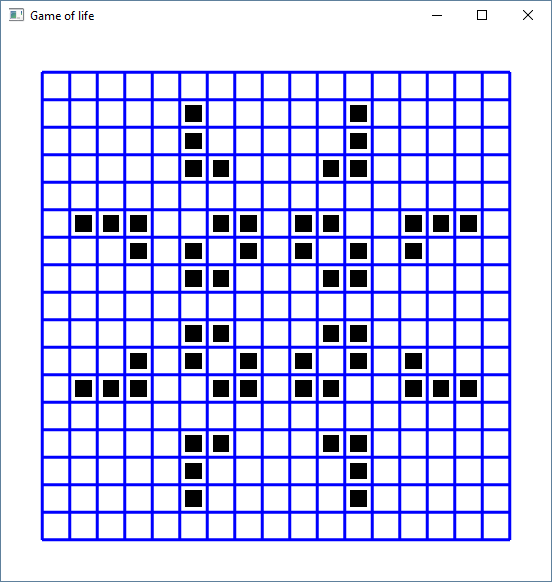
\includegraphics[width=.9\textwidth]{img/cap2_ex9.png}}
        \caption{1ª geração.}
        \label{fig:cap03_ex9a}
    \end{subfigure}
    ~
    \begin{subfigure}[t]{0.27\textwidth}
        \centerline{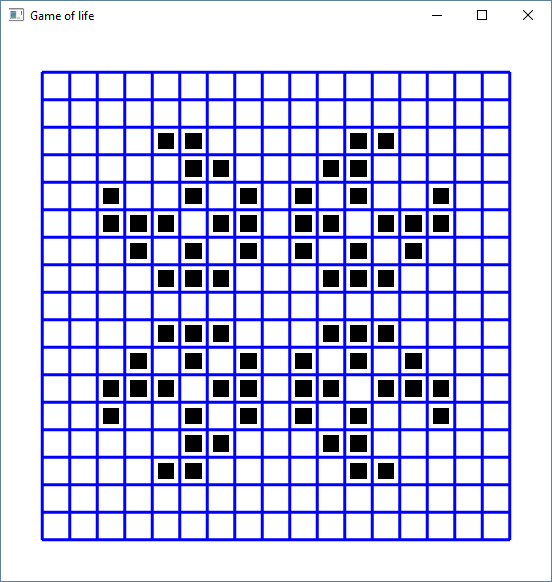
\includegraphics[width=.9\textwidth]{img/cap2_ex9b.png}}
        \caption{2ª geração.}
        \label{fig:cap03_ex9a}
    \end{subfigure}
    ~
    \begin{subfigure}[t]{0.27\textwidth}
        \centerline{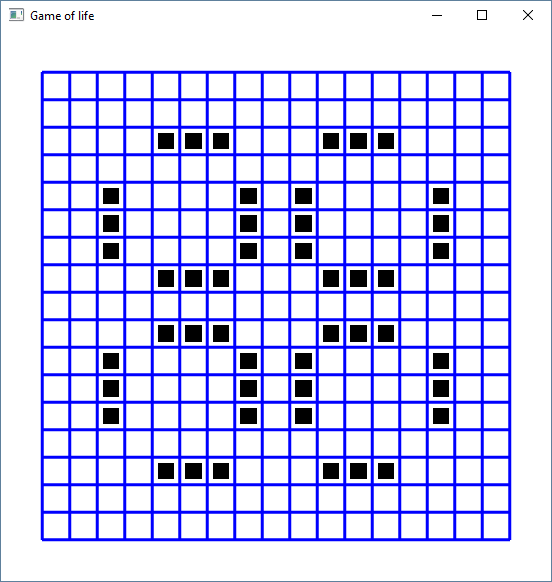
\includegraphics[width=.9\textwidth]{img/cap2_ex9c.png}}
        \caption{3ª geração.}
        \label{fig:cap03_ex9a}
    \end{subfigure}
    \caption{Jogo da vida: a) Primeira geração; b) Segunda geração; c) Terceira geração.}
  \end{figure}

  Comentário: Esta prática mostra como utilizar o retorno das função \emph{CriaQuadrado}, que esta retorna o índice da geometria criada. O seu índice é utilizado na função \emph{Pintar}, que recebe, além do índice, o tipo da geometria. Como foi utilizado a função \emph{CriaQuadrado}, o tipo de geometria é \emph{QUADRADO}. Se fosse utilizado \emph{CriaCirculo}, seria utilizado o tipo \emph{CIRCULO} e assim sucessivamente.
%\lstinputlisting[caption=Código fonte do jogo da vida, style=code, label=lst:cap2_ex2]{src/ex9_gameoflife.cpp}

  \item)
  Implementar o filtro de média móvel para uma matriz M de inteiros (de 0 a 255) com 3 planos RGB, cada um com 100 linhas e 100 colunas.
A matriz a ser filtrada é a imagem uma imagem BMP do Mario. Ela deve ser lida e em seguida mostrada na tela do computador. A imagem filtrada deve igualmente ser apresentada na tela do computador.
  \label{ex:cap02_ex27}

  \begin{figure}[H]
    \centerline{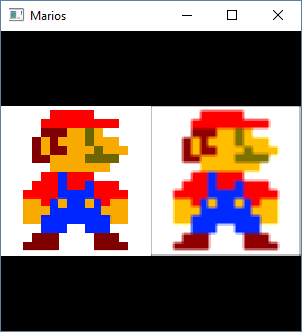
\includegraphics[width=.3\textwidth]{img/cap2_ex27.png}}
    \caption{Filtro Motion Blur.}
    \label{fig:cap02_ex27}
  \end{figure}

Comentário: Esta prática exercita conceitos de processamento de imagens, com manipulação de componentes RGB, agora distribuídos em uma matriz. Os componentes RGB são extraídos de uma imagem bitmap de 24 bits.

%\lstinputlisting[caption=Código fonte do filtro motion blur, style=code, label=lst:cap2_ex27]{src/ex27_mario_filtrado.cpp}

  \item)
  O jogo batalha naval é um jogo de tabuleiro no qual os jogadores devem adivinhar em quais posições do tabuleiro estão localizados os navios do adversário. Ganha aquele que derrubar todos os navios.
Implemente o jogo batalha naval utilizando a \playAPC{}, utilizando as seguintes premissas:
\begin{itemize}
  \item O tabuleiro será 9x9;
  \item Posicione arbitrariamente 10 navios sobre este tabuleiro, sendo 3 navios com tamanho igual a 3, 3 navios com tamanho igual a 2 e 4 navios com tamanho igual a 1;
  \item Não pode posicionar um navio onde já existir outro navio e não pode posicionar o navio imediatamente do lado de outro navio: deve existir pelo menos um espaço vazio entre os dois navios;
  \item Os navios podem estar nas verticais e nas horizontais, não nas diagonais;
  \item Se um navio de tamanho igual a 1 for atingido, fica indicado no lugar que o navio foi derrubado;
  \item Se um navio de tamanho igual a 2 ou 3 for atingido, deve ficar indicado que o navio foi atingido, porém não foi derrubado. Somente quando todas as peças deste navio forem atingidas é que deve-se indicar o navio foi derrubado;
  \item Se o usuário escolheu uma posição do tabuleiro onde não há navio, deve ficar indicado que o usuário não atingiu água e;
  \item O jogo deve avisar ao usuário quando ele conseguir derrubar todos os 10 navios.
\end{itemize}

\label{ex:cap02_ex29}
    \begin{figure}[H]
    \centering
    \begin{subfigure}[t]{0.3\textwidth}
        \centerline{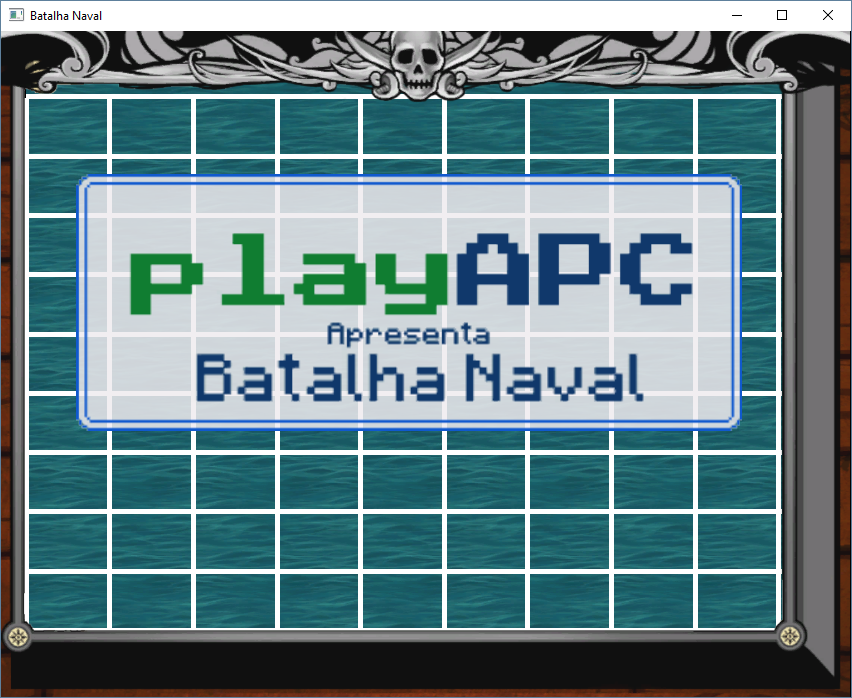
\includegraphics[width=.9\textwidth]{img/cap2_ex29.png}}
        \caption{Tela inicial.}
        \label{fig:cap03_ex26}
    \end{subfigure}
    ~
    \begin{subfigure}[t]{0.3\textwidth}
        \centerline{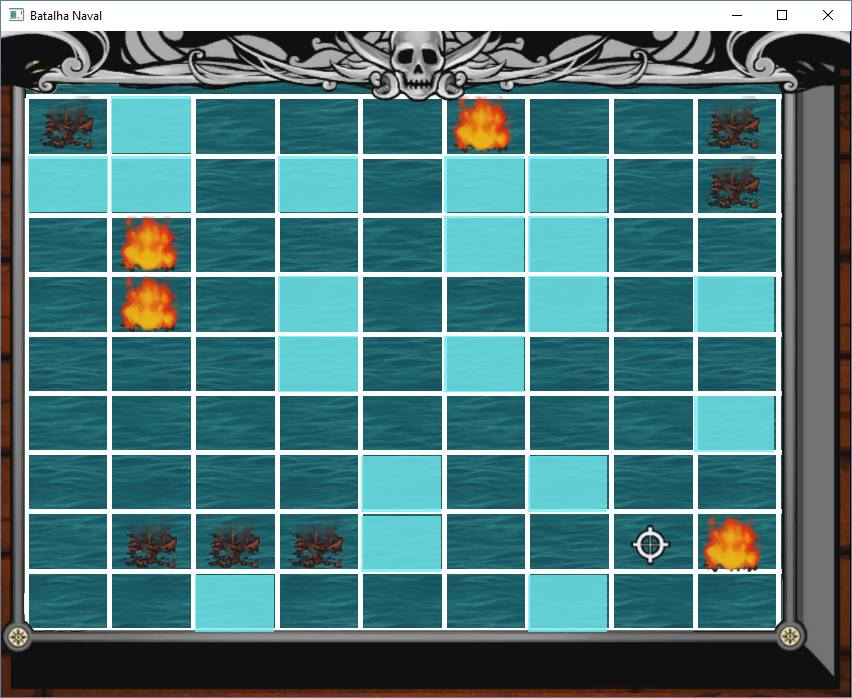
\includegraphics[width=.9\textwidth]{img/cap2_ex29b.png}}
        \caption{Decorrer do jogo: há navios atingidos e navios derrubados.}
        \label{fig:cap03_ex26b}
    \end{subfigure}
    ~
    \begin{subfigure}[t]{0.3\textwidth}
        \centerline{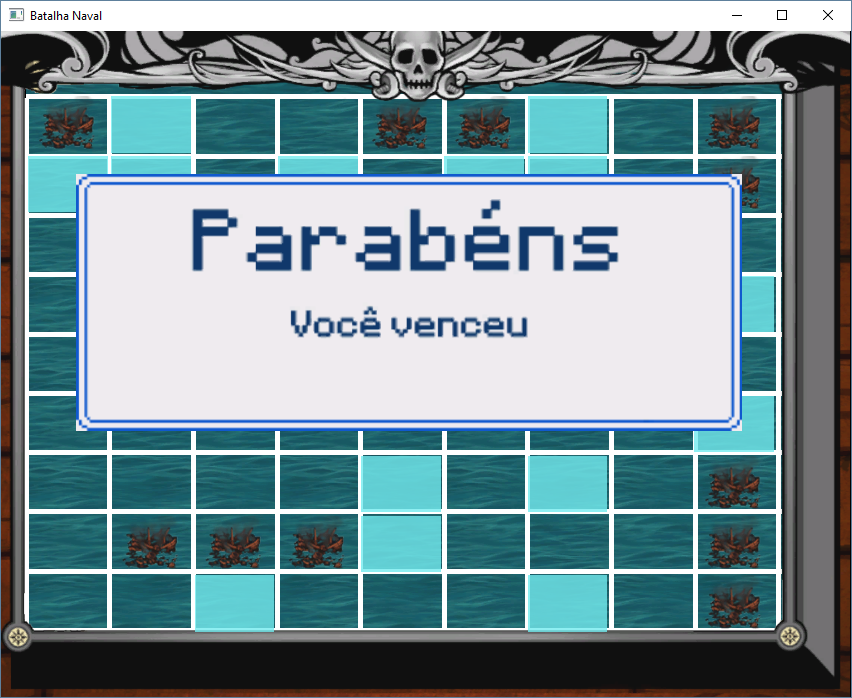
\includegraphics[width=.9\textwidth]{img/cap2_ex29c.png}}
        \caption{Fim do jogo.}
        \label{fig:cap03_ex26c}
    \end{subfigure}
    \caption{Batalha Naval: a) Início; b) Decorrer do jogo; c) Fim do jogo.}
  \end{figure}

Comentário: Esta prática ilustra como as funções \emph{PosicaoMouse}, \emph{ApertouBotaoMouse} e \emph{AssociaImagem} podem ser utilizadas. O aluno deve realizar cálculos para descobrir se o mouse está dentro de uma determinada região da tela e trocar imagens de acordo com a situação do jogo: se o usuário só está posicionando a mira, se o usuário atingiu um navio ou se derrubou um navio.

%\lstinputlisting[caption=Código fonte da batalha naval, style=code, label=lst:cap2_ex29]{src/ex29_batalha.cpp}

\end{renumerate}

\subsection{Subalgoritmos}

\begin{renumerate}
\item)
Crie dois retângulos e posicione-os aleatoriamente em $x$. Coloque uma circunferência no topo do primeiro retângulo e receba do usuário dois valores: ângulo e velocidade. Dado estes valores, calcule e exiba a trajetória balística da circunferência sendo lançada para o outro retângulo. Exiba mensagem caso o usuário consiga acertar o prédio ou não e, em seguida, caso o usuário deseje jogar novamente, sorteie novas posições para os retângulos e execute novamente o procedimento de pedir valores do usuário e exibir a trajetória balística.

  \begin{figure}[ht]
    \centerline{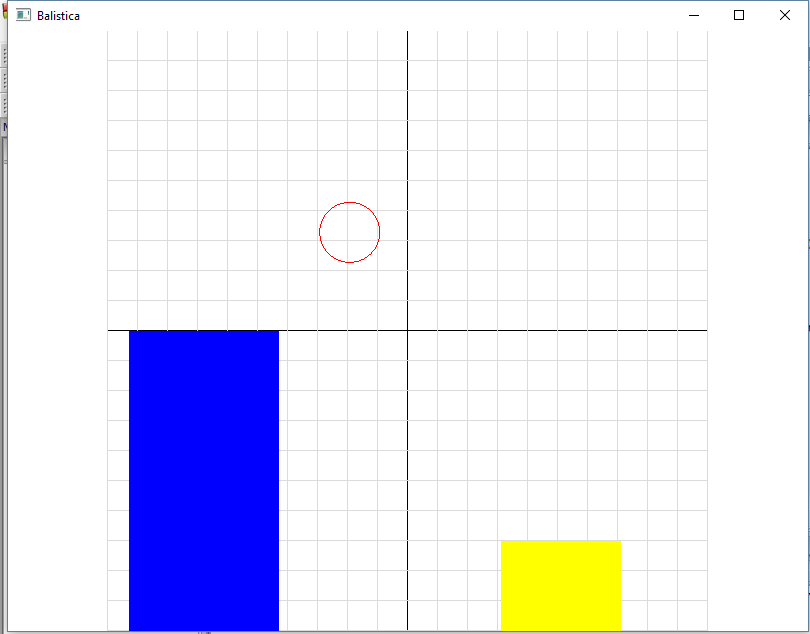
\includegraphics[width=.25\textwidth]{img/cap3_ex12.png}}
    \caption{Lançador Balístico.}
    \label{fig:cap03_ex2}
  \end{figure}

 Comentário: Esta prática ilustra como a função \emph{LimpaDesenho} é usada para poder redesenhar outras cenas.
 \label{ex:cap03_ex1}
%\lstinputlisting[caption=Código fonte do lançador balístico, style=code, label=lst:cap3_ex1]{src/ex12_balistica.cpp}

  \item)
  Baseado no exercício anterior, faça o Wolverine ser lançado de um prédio, dado um ângulo e uma velocidade inicial, com o objetivo de atacar o Magneto. Se não atingir o Magneto, os dois inimigos se encaram. Se atingir o Magneto, faça o Magneto contra-atacar o Wolverine, lançando o mutante em uma trajetória retilínia na direção contrária ao ataque.


   \begin{figure}[H]
    \centering
    \begin{subfigure}[t]{0.25\textwidth}
        \centerline{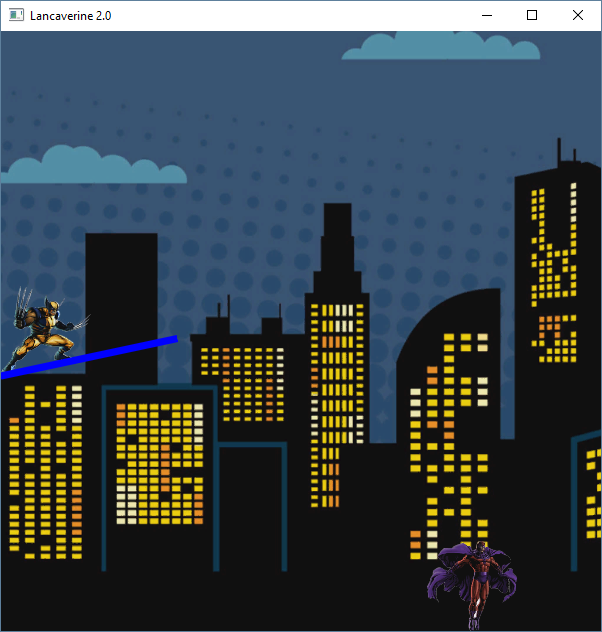
\includegraphics[width=.9\textwidth]{img/cap3_ex27}}
        \caption{Determinação do ângulo.}
        \label{fig:cap03_ex27a}
    \end{subfigure}
    \hfill
    \begin{subfigure}[t]{0.25\textwidth}
        \centerline{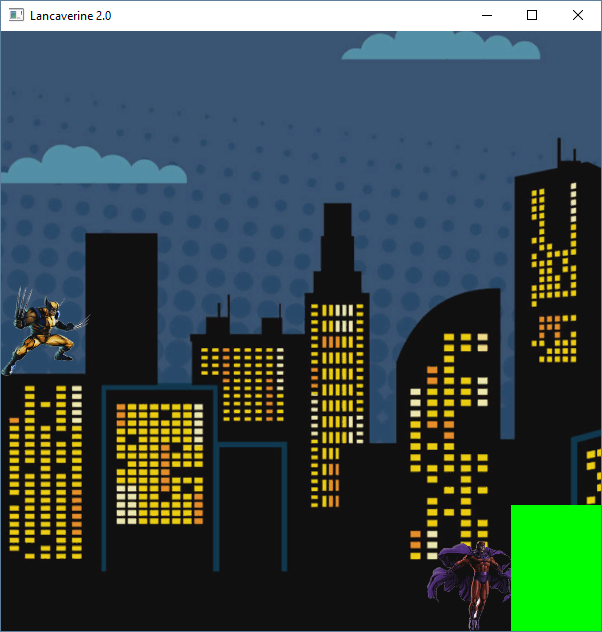
\includegraphics[width=.9\textwidth]{img/cap3_ex27b}}
        \caption{Determinação da velocidade inicial.}
        \label{fig:cap03_ex27b}
    \end{subfigure}
    \hfill
    \begin{subfigure}[t]{0.25\textwidth}
        \centerline{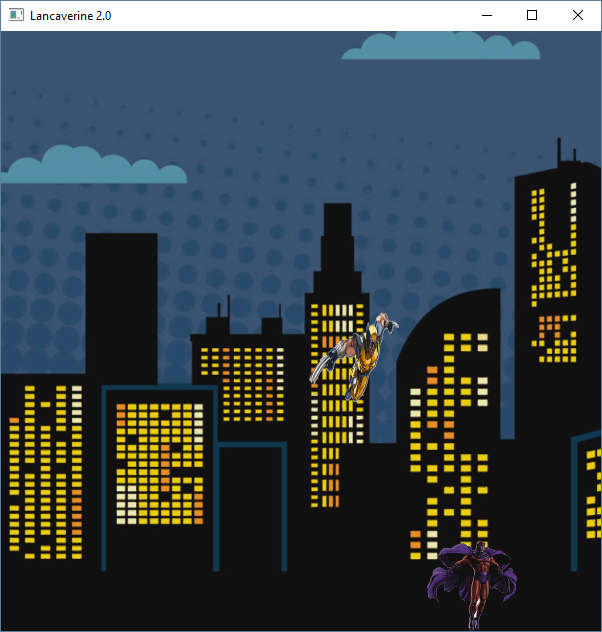
\includegraphics[width=.9\textwidth]{img/cap3_ex27c}}
        \caption{Wolverine sendo lançado.}
        \label{fig:cap03_ex27c}
    \end{subfigure}
    \hfill
    \begin{subfigure}[t]{0.25\textwidth}
        \centerline{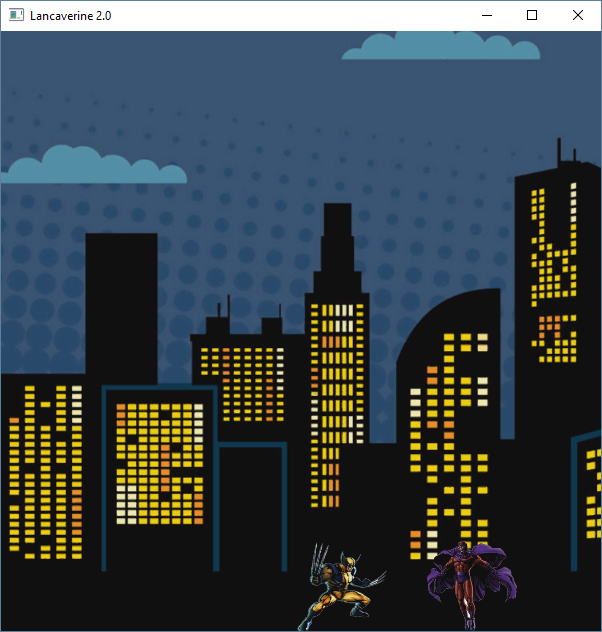
\includegraphics[width=.9\textwidth]{img/cap3_ex27d}}
        \caption{Wolverine e Magneto se encarando.}
        \label{fig:cap03_ex27d}
    \end{subfigure}
    ~
    \begin{subfigure}[t]{0.25\textwidth}
        \centerline{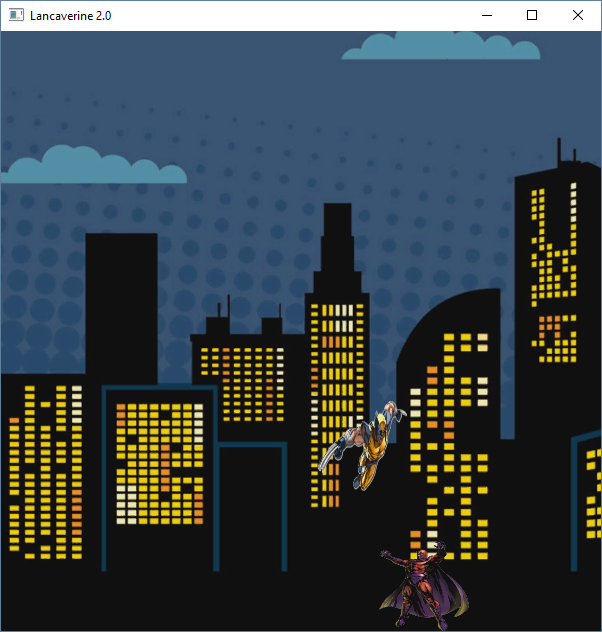
\includegraphics[width=.9\textwidth]{img/cap3_ex27e}}
        \caption{Wolverine sendo lançado pelo Magneto.}
        \label{fig:cap03_ex27e}
    \end{subfigure}

    \caption{Lançaverine: a) Ângulo de lançamento; b) Velocidade inicial; c) Wolverine percorrendo trajetória; d) Caso quando Wolverine não acerta o Magneto; e) Caso quando Wolverine acerta o Magneto.}

  \end{figure}

  \label{ex:cap03_ex27} 
  Comentário: Esta prática exercita o conceito de animação. Ela também ilustra como utilizar o conceitos de grupos na \playAPC{} de forma mais eficiente, liberando espaço na memória quando um grupo não é mais utilizado, como o grupo \emph{lancar}, na Listagem \ref{lst:cap3_ex27}.
%\lstinputlisting[caption=Código fonte do Lançaverine, style=code, label=lst:cap3_ex27]{src/ex28_lancaverine.cpp} 
  
\item)
Snake foi um jogo que começou no console Atari, em 1976, e foi popularizado nos anos 90 quando a Nokia começou a colocar o jogo em seus celulares. 
  
  O jogador controla uma cobra, que é representada por um quadrado no começo, e, a cada novo alimento que a cobra ingere, ela aumenta em um quadrado o seu tamanho, aumentando gradativamente a dificuldade do jogo. Se a cobra atingir a parede, ela morre. Se a cobra atingir o próprio corpo, ela também morre.

  Dado estas regras, crie uma versão do jogo Snake utilizando a \playAPC.

  \label{ex:cap03_ex2}

  \begin{figure}[H]
    \centerline{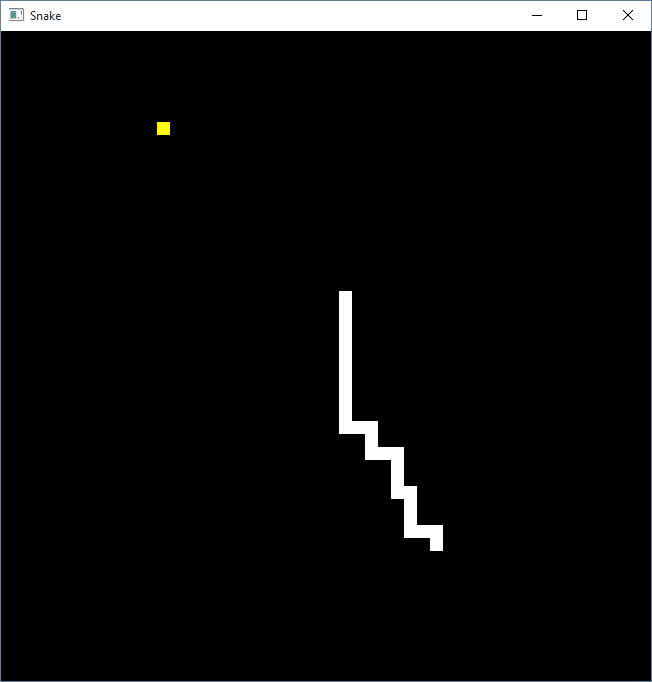
\includegraphics[width=.25\textwidth]{img/cap3_ex10.png}}
    \caption{Jogo Snake.}
    \label{fig:cap03_ex2}
  \end{figure}
 Comentário: Esta prática ilustra como a função \emph{ApertaTecla} e \emph{MudaLimitesJanela} podem ser utilizadas: a primeira para lidar com input de teclado \footnote{\url{http://playapc.zaghetto.com/funcoes/extras/input/tecla-pressionada}} e a segunda para ajustar o plano onde as geometrias serão desenhadas.
%\lstinputlisting[caption=Código fonte de Snake, style=code, label=lst:cap3_ex1]{src/ex10_snake.cpp}

\end{renumerate}

\subsection{Recursão}

\begin{renumerate}

\item)
Construa uma árvore binária recursiva onde o usuário oferece altura, profundidade e ângulo entre ramos. A árvore deverá ser construída tanto para o lado esquerdo, com ângulo entre os galhos de $\theta$ fornecida pelo usuário, quanto para o lado direito, com ângulo $-\theta$.
  \label{ex:cap04_ex2}

  \begin{figure}[H]
    \centerline{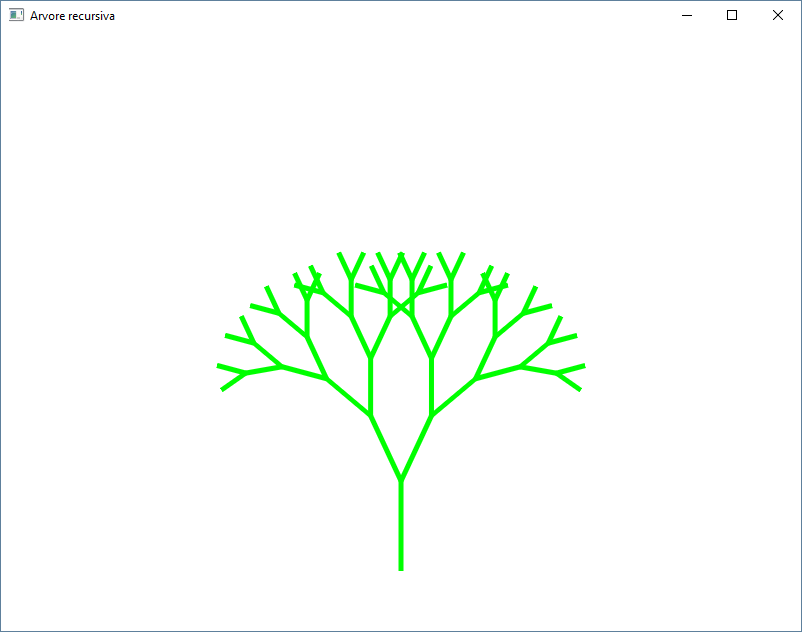
\includegraphics[width=.3\textwidth]{img/cap4_ex17.png}}
    \caption{Árvore Binária com altura $30$, ângulo $25$º e profundidade $6$.}
    \label{fig:cap04_ex2}
  \end{figure}

  Comentário: Esta prática reforça que os valores da estrutura \emph{Ponto} podem ser ponto flutuantes.
%\lstinputlisting[caption=Árvore recursiva, style=code, label=lst:cap4_ex3]{src/ex17_arvore.cpp}

\item)
Torre de Hanói é um jogo matemático onde seu objetivo é passar os discos de uma torre $A$ para uma torre $B$, utilizando uma torre $C$ como auxiliar. Ele segue as seguintes regras:
  \begin{enumerate}
    \item Só pode mover um disco de cada vez
    \item Só pode mover o disco que estiver mais acima de uma torre e deve-se colocar no topo de outra torre
    \item Não é permitido colocar um disco de tamanho maior em cima de um disco de tamanho menor
  \end{enumerate}

  Ilustre a resolução da torre de Hanói para uma quantidade de 5 discos ou menos.
  \label{ex:cap04_ex1}

  \begin{figure}[H]
    \centerline{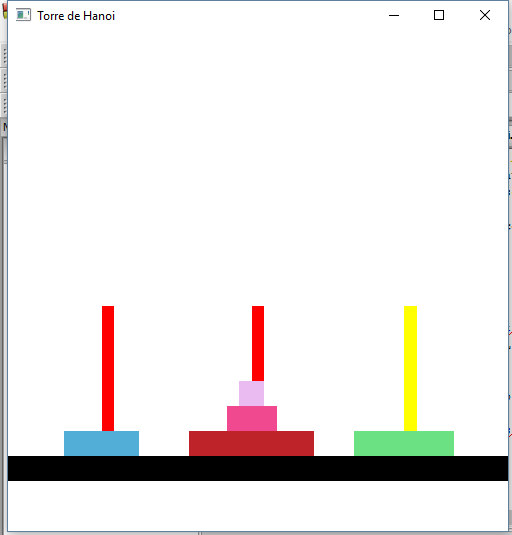
\includegraphics[width=.3\textwidth]{img/cap4_ex13.png}}
    \caption{Solucionador da torre de Hanói.}
    \label{fig:cap04_ex1}
  \end{figure}

  Comentário: Esta prática ilustra como mover cada geometria utilizando retorno da função \emph{CriaGrupo} para mover cada peça da torre de Hanoi para uma posição específica.

\item)
Sabe-se que a curva de Koch começa sendo construída com um segmento de reta de tamanho $\frac{n}{3}$. Na extremidade deste primeiro segmento, desenha-se outro segmento de reta de tamanho $\frac{n}{3}$, porém com uma curvatura de $60º$ em relação ao primeiro. Na extremidade deste segundo segmento, desenha-se outra curva de reta de tamanho $\frac{n}{3}$, mas agora com a curvatura de $120º$ em relação ao primeiro. Por fim, desenha-se outro segmento de reta de tamanho $\frac{n}{3}$ na extremidade do terceiro segmento, sem diferença de curvatura.
    \mbox{}\\
    \begin{enumerate}[label=(\alph*)]
      \item 
      Exiba a curva de Koch de ordem $i$ com tamanho $n$ igual à $180$ unidades centrada na posição $(-100, 0)$. 
        
        (NOTA: a partir de um certo nível de recursão, é possível que a divisão dos segmentos de retas comecem a dividir pixels, tornando inviável a visualização)

      Como sugestão, a Listagem \ref{func:koch} exemplifica um cabeçalho da função \emph{koch}, onde seu primeiro argumento é o ponto de origem, seu segundo argumento é o tamanho do segmento de reta, seu terceiro argumento é a inclinação do segmento e seu quarto argumento é a ordem da curva. A função retorna o segundo ponto da reta naquele nível de recursão que deverá ser criada.

      \begin{lstlisting}[caption=Header da função koch, label={func:koch},numbersep=0pt,resetmargins=true, language=C++]
      Ponto koch (Ponto from, double len, double theta, int order)
      \end{lstlisting}

        \label{ex:cap04_ex3a}

          \begin{figure}[H]
          \centering
          \begin{subfigure}[t]{0.3\textwidth}
              \centerline{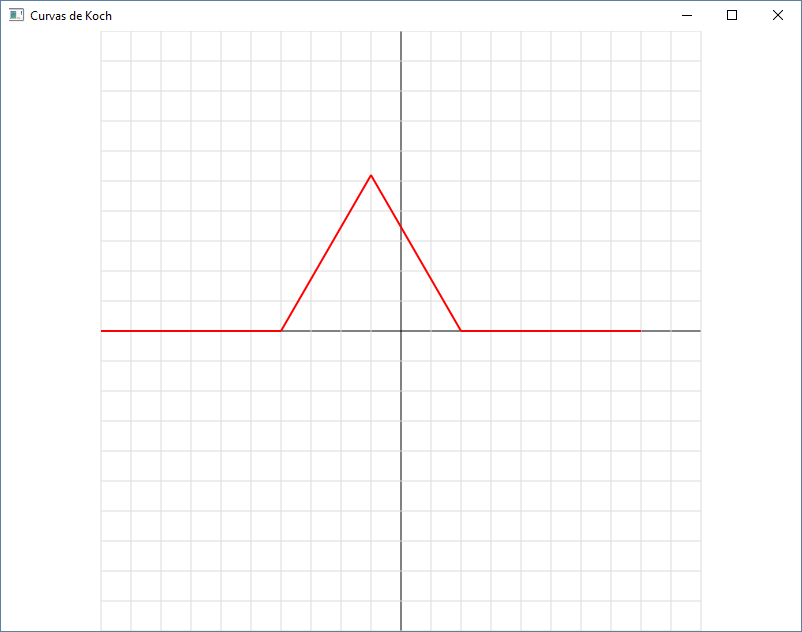
\includegraphics[width=.9\textwidth]{img/cap4_ex14}}
              \caption{Curva de Koch de ordem $1$.}
              \label{fig:cap03_ex14a}
          \end{subfigure}
          \hfill
          \begin{subfigure}[t]{0.3\textwidth}
              \centerline{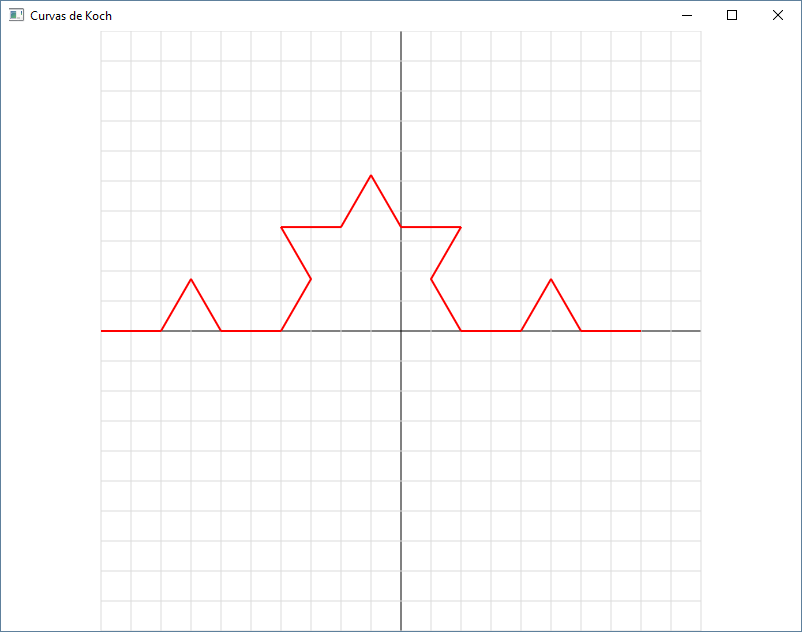
\includegraphics[width=.9\textwidth]{img/cap4_ex14b}}
              \caption{Curva de Koch de ordem $2$.}
              \label{fig:cap03_ex14b}
          \end{subfigure}
          \hfill
          \begin{subfigure}[t]{0.3\textwidth}
              \centerline{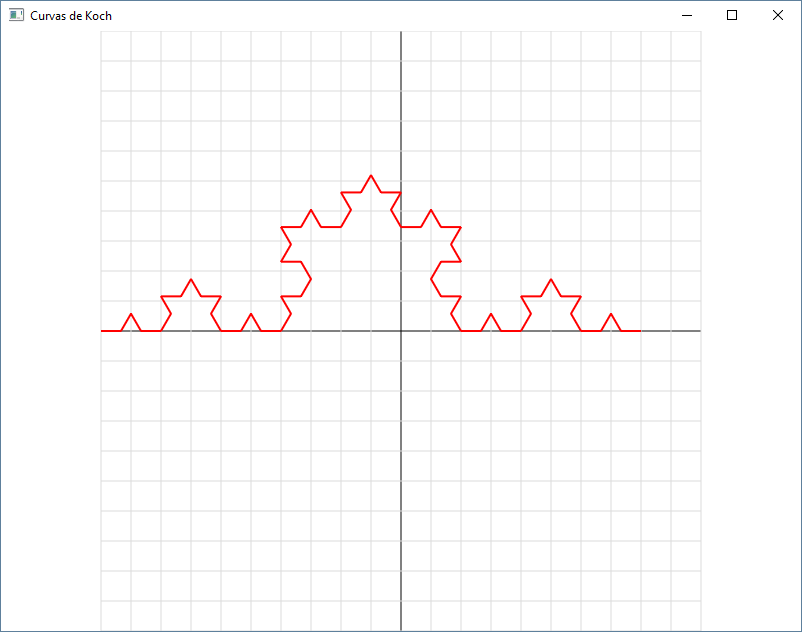
\includegraphics[width=.9\textwidth]{img/cap4_ex14c}}
              \caption{Curva de Koch de ordem $3$.}
              \label{fig:cap03_ex14c}
          \end{subfigure}
          \hfill
          \begin{subfigure}[t]{0.3\textwidth}
              \centerline{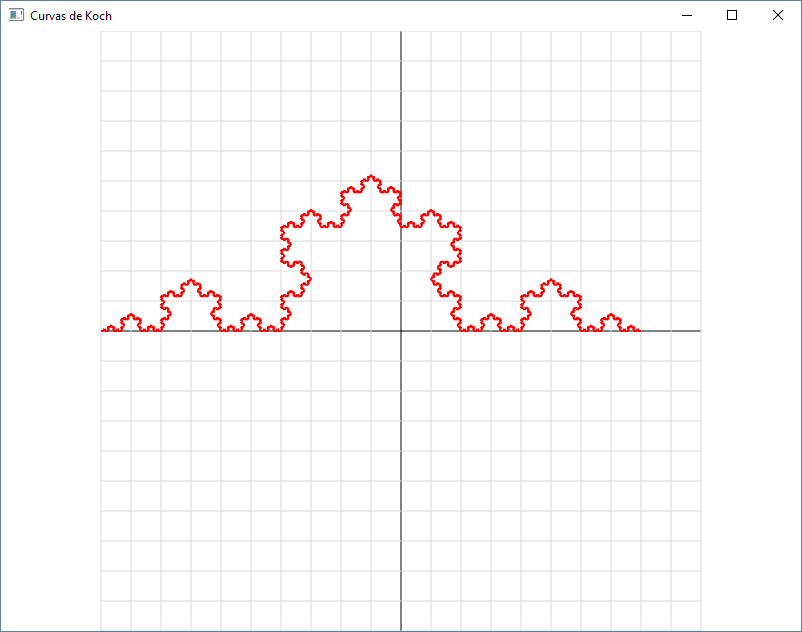
\includegraphics[width=.9\textwidth]{img/cap4_ex14d}}
              \caption{Curva de Koch de ordem $6$.}
              \label{fig:cap03_ex14d}
          \end{subfigure}
          
          \caption{
            \label{fig:koch}%
            Curva de Koch: a) Ordem 1; b) Ordem 2; c) Ordem 3; d) Ordem 6.
          }

        \end{figure}

  \label{ex:cap03_ex27}
      Comentário: Esta prática reforça o modo de utilização da função \emph{CriaReta}, usando a função \emph{movaCaneta}.
%\lstinputlisting[caption=Código fonte da curva de koch, style=code, label=lst:cap4_ex2a]{src/ex14_koch.cpp}

      \item 
      Utilize a curva de Koch criada no item anterior para criar outras duas curvas, com uma diferença de angulação: a primeira curva será criada da mesma maneira no item anterior; a segunda curva será inclinada em $120º$ e; a terceira curva será inclinada em $-120º$. 

      As Figuras \ref{fig:flocos} ilustram as três retas, onde a primeira curva, com inclinação $0º$, está representada em vermelho, a segunda, com inclinação de $120º$ está representada em verde e a terceira curva, com inclinação $-120º$ está representada em azul.
      \label{ex:cap04_ex3b}

      \begin{figure}[H]
          \centering
          \begin{subfigure}[t]{0.3\textwidth}
              \centerline{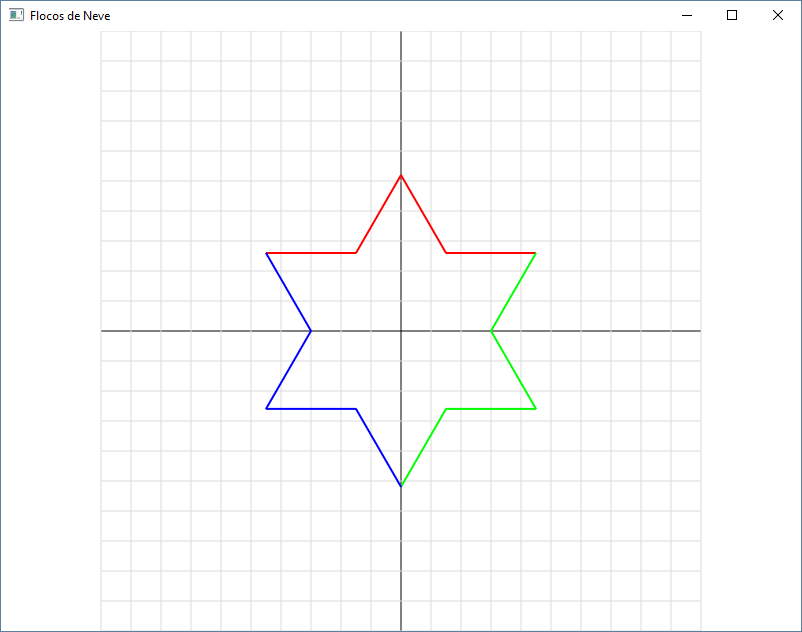
\includegraphics[width=.9\textwidth]{img/cap4_ex15}}
              \caption{Floco de neve de ordem $1$.}
              \label{fig:cap04_ex15a}
          \end{subfigure}
          \hfill
          \begin{subfigure}[t]{0.3\textwidth}
              \centerline{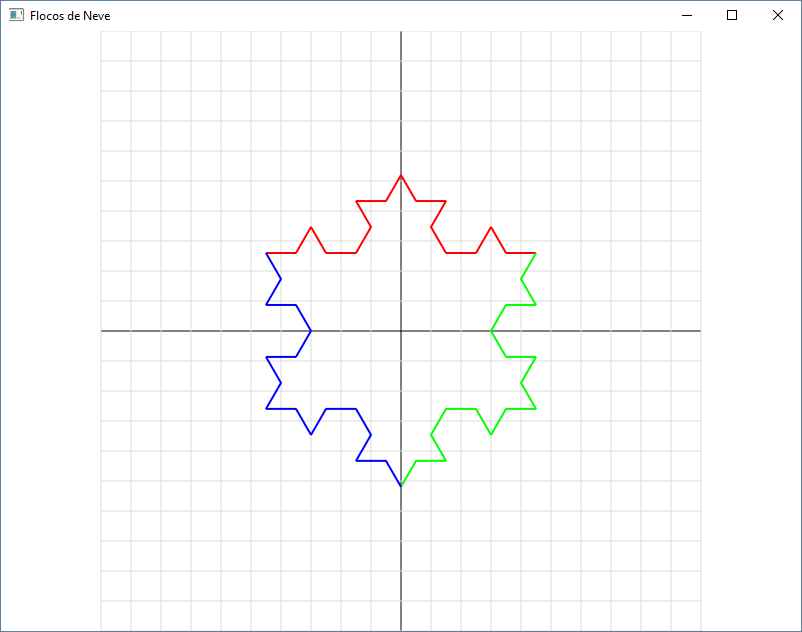
\includegraphics[width=.9\textwidth]{img/cap4_ex15b}}
              \caption{Floco de neve de ordem $2$.}
              \label{fig:cap04_ex15b}
          \end{subfigure}
          \hfill
          \begin{subfigure}[t]{0.3\textwidth}
              \centerline{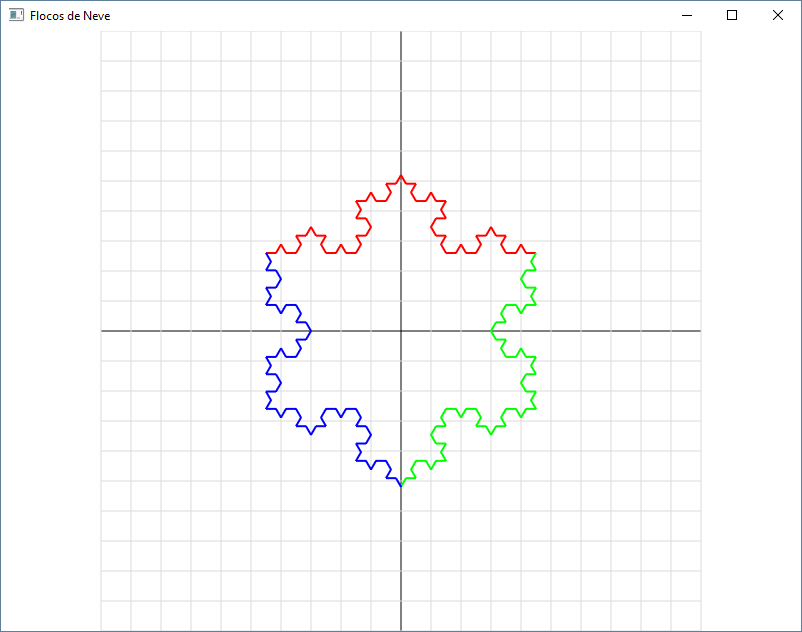
\includegraphics[width=.9\textwidth]{img/cap4_ex15c}}
              \caption{Floco de neve de ordem $3$.}
              \label{fig:cap04_ex15c}
          \end{subfigure}
          \hfill
          \begin{subfigure}[t]{0.3\textwidth}
              \centerline{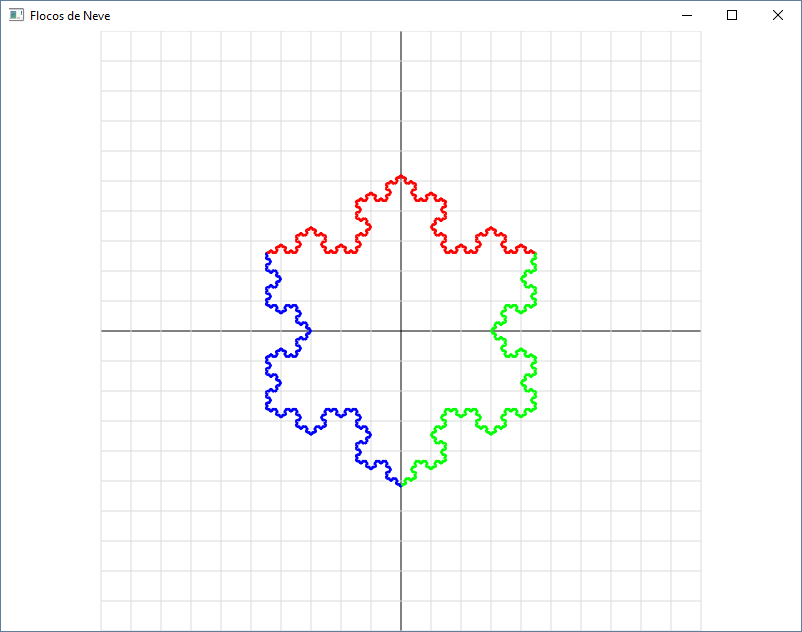
\includegraphics[width=.9\textwidth]{img/cap4_ex15d}}
              \caption{Floco de neve de ordem $6$.}
              \label{fig:cap04_ex15d}
          \end{subfigure}

          \caption{
            \label{fig:flocos}%
            Floco de neve: a) Ordem 1; b) Ordem 2; c) Ordem 3; d) Ordem 6.
          }

        \end{figure}
        Comentário: Esta prática é uma evolução do exercício anterior.
%\lstinputlisting[caption=Código fonte do floco de neve, style=code, label=lst:cap4_ex2b]{src/ex15_snowflake.cpp}
    \end{enumerate}
    \label{ex:cap04_ex3}

\item)
 A curva de Sierpiński é uma curva do tipo \emph{space-filling curve}, a qual significa que ela tenta ocupar todo espaço disponível sem ser cruzar. Ela pode ser implementada utilizando quatro funções mutuamente recursivas, \emph{A, B, C} e \emph{D}. A Figura \ref{fig:cap04_ex16} ilustra essa curva com as 4 curvas básicas. A curva A está representado em vermelho, a curva B em verde, a curva C em azul e a curva D em amarelo, sendo as curvas que conectam estas 4 curvas básicas representadas em preto.

   \begin{figure}[H]
    \centerline{\includegraphics[width=1.0\textwidth]{img/cap4_ex16.png}}
    \caption{Curva de Sierpiński de ordem $1$ com ângulo de $45º$.}
    \label{fig:cap04_ex16}
  \end{figure}


 O programa inicia com uma curva básica \emph{S} dada pelo padrão A 
      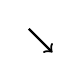
\begin{tikzpicture}
        \draw[thick,->] (0.0,0.30) -- (0.30,0.0);
      \end{tikzpicture}
      , B
      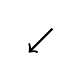
\begin{tikzpicture}
        \draw[thick,->] (0.30,0.30) -- (0.0,0.0);
      \end{tikzpicture}
      , C
      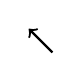
\begin{tikzpicture}
        \draw[thick,->] (0.30,0.0) -- (0.0,0.30);
      \end{tikzpicture}
      e D
      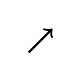
\begin{tikzpicture}
        \draw[thick,->] (0.0,0.0) -- (0.30,0.30);
      \end{tikzpicture}
      . As setam indicam a virada do ângulo que as retas \emph{fecham} os desenhos das funções.
  \begin{itemize}
    \item
      A curva A é dada pelo padrão A
      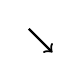
\begin{tikzpicture}
        \draw[thick,->] (0.0,0.30) -- (0.30,0.0);
      \end{tikzpicture}
      , B
      \begin{tikzpicture}
        \draw[thick,->] (0.0,0.0) -- (0.30,0.0);
      \end{tikzpicture}
      , D
      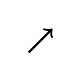
\begin{tikzpicture}
        \draw[thick,->] (0.0,0.0) -- (0.30,0.30);
      \end{tikzpicture}
      A
    \item
      A curva B é dada pelo padrão B
      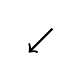
\begin{tikzpicture}
        \draw[thick,->] (0.30,0.30) -- (0.0,0.0);
      \end{tikzpicture}
      , C
      \begin{tikzpicture}
        \draw[thick,->] (0.30,0.30) -- (0.30,0.0);
      \end{tikzpicture}
      , A
      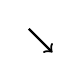
\begin{tikzpicture}
        \draw[thick,->] (0.0,0.30) -- (0.30,0.0);
      \end{tikzpicture}
      B
    \item
      A curva C é dada pelo padrão C
      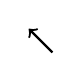
\begin{tikzpicture}
        \draw[thick,->] (0.30,0.0) -- (0.0,0.30);
      \end{tikzpicture}
      , D
      \begin{tikzpicture}
        \draw[thick,->] (0.30,0.0) -- (0.0,0.0);
      \end{tikzpicture}
      , B
      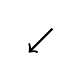
\begin{tikzpicture}
        \draw[thick,->] (0.30,0.30) -- (0.0,0.0);
      \end{tikzpicture}
      C
    \item
      A curva D é dada pelo padrão D
      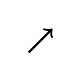
\begin{tikzpicture}
        \draw[thick,->] (0.0,0.0) -- (0.30,0.30);
      \end{tikzpicture}
      , A
      \begin{tikzpicture}
        \draw[thick,->] (0.30,0.0) -- (0.30,0.30);
      \end{tikzpicture}
      , C
      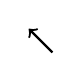
\begin{tikzpicture}
        \draw[thick,->] (0.30,0.0) -- (0.0,0.30);
      \end{tikzpicture}
      D
  \end{itemize}
  Considere o ângulo de inclinação da curva de Sierpiński como $45º$, ou seja, as retas desenhadas tem uma inclinação de $45º$ entre si. Considere também que a curva tenha uma altura $h$ de $40$ unidades e que, caso a ordem de recusão $n$ seja maior que $0$, a altura será determinada por $\frac{h}{n^{2}}$. A criação das curvas se inicia no ponto $p$ em $(-70, 100)$. 

  Considere que a Listagem \ref{func:sier} seja a função que calcula o próximo ponto baseando no ângulo de inclinação e desenha esta reta. Estes fatores são passados de acordo com a Listagem \ref{func:mainsier}.
  \label{ex:cap04_ex4}

  \begin{lstlisting}[caption={Função para conectar próxima curva}, style=tuto, , label={func:sier}] 
      Ponto reta(int fator, int h, Ponto p) {
        // ang é para multiplicar por 45 graus
        Ponto p1;
        double ar = fator * 45.0 * PI/180;

        p1.x = p.x + h*cos(ar);
        p1.y = p.y + h*sin(ar);
        CriaReta(p,p1);
        Grafite(2);
        Pintar(0,0,255);
        return p1;
      }
      \end{lstlisting}

    \begin{lstlisting}[caption={Função main Curva de Sierpiński}, style=tuto, label={func:mainsier}] 
      int main() {

        Ponto p;
        int   k; 
        float   h = 40;

        printf("Insira a ordem para a criacao das curvas: ");
        scanf("%d", &k);

        p.x = -70; p.y = 100; //ordem=1 cabe todo na tela


        MostraPlanoCartesiano(10);
        AbreJanela(800,600, "Curvas de Sierpinski");
        PintarFundo(255, 255, 255);


        if (k>0) h /= k*k;
        p = A(k,h, p); 
        p = reta(7,h, p); //calcula o proximo ponto onde a outra reta deve comecar

        p = B(k,h, p); 
        p = reta(5,h, p); 

        p = C(k,h, p); 
        p = reta(3,h, p);

        p = D(k,h, p); 
        p = reta(1,h, p);

        Desenha();

        return 0;
      }
      \end{lstlisting}

  Implemente as funções $A$, $B$, $C$ e $D$ da curva de Sierpiński.

  \begin{figure*}[!htp]
          \centering
          \begin{subfigure}[t]{0.45\textwidth}
              \centerline{\includegraphics[width=.9\textwidth]{img/cap4_ex16b}}
              \caption{Curva de Sierpiński de ordem $2$.}
              \label{fig:cap03_ex14a}
          \end{subfigure}
          \hfill
          \begin{subfigure}[t]{0.45\textwidth}
              \centerline{\includegraphics[width=.9\textwidth]{img/cap4_ex16c}}
              \caption{Curva de Sierpiński de ordem $3$.}
              \label{fig:cap03_ex14b}
          \end{subfigure}
          
          \caption{
            \label{fig:koch}%
            Curva de Sierpiński: a) Ordem 2; b) Ordem 3.
          }

        \end{figure*}
  Comentário: Esta prática reforça o modo de utilizar a função \emph{CriaReta}. Além disso, exercita fundamentalmente recursões mútuas entre 4 funções.
%\lstinputlisting[caption=Código fonte da curva de Sierpiński, style=code, label=lst:cap4_ex1]{src/ex16_sierpinski.cpp}
  
\end{renumerate}

















\section{Aceitação por parte dos professores em participar do experimento de aplicar a \playAPC}

Assim que a \playAPC{} passou a ter versões estáveis para o uso, professores envolvidos com o projeto passaram a criar seus próprios materiais (Anexo \ref{attachment:recursaoRalha}) e a desenvolver suas próprias práticas. Todos os exercícios de recursão foram desenvolvidos pelo Professor Ralha, exceto o \ref{ex:cap04_ex1}. Além destes, outros diversos exercícios também foram propostos e testados pelo professor, como o da espiral hiperbólica, \ref{ex:cap01_ex5}, o do moinho de vento, \ref{ex:cap01_ex7} e grande parte dos exercícios extras disponíveis na Apostila (Apêndice \ref{appendix:apostila}). Nas versões mais recentes da \playAPC{}, o professor Alexandre Zaghetto utilizou a biblioteca para programar exemplos do autômato Jogo da Vida \footnote{\url{https://www.youtube.com/watch?v=hel1VwfLJDM}} \footnote{\url{https://www.youtube.com/watch?v=96KXQERnsis}} e também criou uma adaptação da obra \emph{Circles in a Circles} do pintor Wassily Kandinsky. Sua adaptação é conhecida como \emph{Sub-Kandisy Generator} \footnote{\url{https://www.youtube.com/watch?v=UlVh9Dw0Sgo}}.

Utilizando a última versão da \playAPC{}, versão 1.7.2, um exercício criado pelo Professor Zaghetto foi o Certificado de Bravura (Anexo \ref{attachment:bravura}). Neste exercício, os alunos tiveram até a Semana Universitária da \acrshort{UnB} para implementar a própria versão do jogo \emph{Freeway}, jogo criado em 1981 e publicado pela empresa Atari.

\section{Aceitação por parte dos alunos}
A \playAPC{} passou a ser aplicada a partir do semestre 2/2014, na turma de \acrshort{CB} orientada pelo Professor Jóse Carlos Loureiro Ralha. Nos semestres 1/2015 e 2/2015, foram aplicadas nas turmas de \acrshort{CB} do Professor Alexandre Zaghetto e da Professora Carla Castanho, ambos utilizando a biblioteca em somente uma prática.

Com a versão 1.7.2 da \playAPC{}, foi aplicada um questionário de satisfação de uso (Anexo \ref{appendix:questionario}) na turma de 2/2016 ministrada pelo Prof. Alexandre Zaghetto, no qual cinco das dez práticas utilizaram a \playAPC{}. O questionário avalia o Guia de Referência, os recursos da biblioteca e se ela cumpriu seu objetivo de auxiliar o ensino. 

\figura[!h]{img/satisfacao}{Gráfico com o balanço geral das respostas dos alunos de \acrshort{APC} das turmas E e H. Respostas em branco foram consideradas com valor $0$}{fig:satisfacao}{width=1.0\textwidth}%
A partir Figura \ref{fig:satisfacao}, é possível inferir que a biblioteca possui uma ótima aceitação, pois: 
\begin{itemize}
  \item Os alunos concordam que:
    \begin{itemize}
       \item O Guia possui uma navegação simples e sua documentação está clara;
       \item Foi fácil utilizar a \playAPC{} nas práticas de algoritmos sequencias, vetores e a realização de um jogo e;
       \item Utilizar a \playAPC{} é mais interessante que utilizar somente a tela do terminal para saída do programa.
    \end{itemize}
  \item Os alunos concordam em parte que:
    \begin{itemize}
      \item Foi fácil utilizar a \playAPC{} na prática de matrizes e;
      \item Utilizar a \playAPC{} ajudou no entendimento da linguagem C.
    \end{itemize}
\end{itemize}
 
 Para a prática de algoritmos sequenciais, os exercícios aplicados foram os de:
   \begin{enumerate}
     \item Exibir um boneco palito, \ref{ex:cap01_ex2};
     \item Exibir a estrela de davi, \ref{ex:cap01_ex3};
     \item Exibir um quadrado inscrito, \ref{ex:cap01_ex8};
     \item Verificar se ponto está dentro ou fora de uma circunferência, \ref{ex:cap01_ex22} e;
     \item Verificar existência de triângulo, \ref{ex:cap01_ex23}.
  \end{enumerate}
  Para a prática de vetores, o exercício aplicado foi o de aplicar filtro de média móvel em um vetor RGB, \ref{ex:cap02_ex26}.
  Para a prática de matrizes, os exercícios aplicados foram os de:
  \begin{enumerate}
     \item Implementar o Jogo da vida, \ref{ex:cap02_ex2};
     \item Aplicar filtro de média móvel em uma imagem, \ref{ex:cap02_ex27}.
  \end{enumerate}
  Para a prática de realizar um jogo, o exercício aplicado foi o Certificado de Bravura (Anexo \ref{attachment:bravura}).

\subsection{Instalação da biblioteca}
Anteriormente, o código fonte da \playAPC{} era anexado ao projeto do aluno e somente a partir daí era usado as funções da biblioteca. Atualmente, o Guia de Referência (Anexo \ref{appendix:guia}) oferece passo a passo da instalação, com vídeo explicando onde colocar a biblioteca de vínculo dinâmico e como linkar a biblioteca utilizando a IDE Code::Blocks.

O principal desafio encontrado pela \playAPC{} é a instalação em computadores que possuem apenas versões da OpenGL 1.0, sendo que a \playAPC{} utiliza funções a partir da versão 1.3. Este problema é contornado atualizando os drivers da placa de vídeo, porém nem todos os alunos possuem facilidade neste processo de atualização.

Outro grande desafio é a instalação da biblioteca em plataformas Mac: devido a falta de hardware compatível e falta de suporte das máquinas virtuais utilizadas, não foi possível a geração de binários. Por conta disso, são entregues ao aluno dois arquivos makefile, um para instalação das dependências e outro para instalação da biblioteca propriamente dita. Porém, não é todo aluno de primeiro semestre que possui um Mac que sabe como utilizar um makefile ou até mesmo utilizar o terminal.

\subsection{Utilização da biblioteca}
Uma das consequências observadas ao utilizar a \playAPC{} por parte dos alunos foi a liberdade criativa que a biblioteca proporciona. Os enunciados, apesar de serem auto-explicativos, não restringem a utilização dos recursos. Todos possuem acesso ao Guia de Referência (Apêndice \ref{appendix:guia}) e, uma vez que suas funções podem ser usadas em qualquer momento do curso, depende somente do grau de criatividade do aluno para deixar a prática mais interessante.

Por exemplo, uma das práticas de algoritmos sequenciais foi a renderização de um boneco palito, \ref{ex:cap01_ex2}, na qual foram sugeridas utilização das geometrias como reta e circunferência para serem utilizadas. Um dos alunos teve a liberdade criativa de fazer, ao invés de um boneco palito padrão, um boneco palito dançando, como ilustra a Figura \ref{fig:lab1}.

 \begin{figure}[H]
 \begin{center}
 \includegraphics[scale=.5]{img/aluno_lab1.png}
 \end{center}
 \caption{Prática 3 de Algoritmos Sequenciais, realizada pelo aluno Bernado Ferreira Santos Ximbre, \acrshort{APC} turma E de 2/2016.}
 \label{fig:lab1}
 \end{figure}

Outro exemplo foi a prática de algoritmo de repetição foi a renderização de hélices girando em torno do centro do plano cartesiano, dando a impressão de um ventilador, \ref{ex:cap01_ex7}. Um dos alunos adicionou um outro contexto na cena e criou um moinho de vento, como ilustra a Figura \ref{fig:lab2}. Mais tarde, esta prática foi reformulada respeitando o contexto criado pelo aluno.

 \begin{figure}[H]
 \begin{center}
 \includegraphics[scale=.25]{img/moinho.png}
 \end{center}
 \caption{Prática 1 de Algoritmos com Repetição, realizada pelo aluno Pedro Paulo de Pinho Matos, \acrshort{CB} turma B de 2/2014.}
 \label{fig:lab2}
 \end{figure}

 Outro exemplo é a prática de vetores, em que dada a entrada de 20 componentes RGB, pedia-se para renderizar os componentes originais e os componentes filtrados, \ref{ex:cap02_ex26}. Foi sugerido a utilização de quadrados alinhados verticalmente, mas não era regra. Um dos alunos exibiu os vetores originais e os filtrados em forma de um círculo, onde o círculo externo são os vetores originais e o círculo interno representa os vetores filtrados.

  \begin{figure}[H]
 \begin{center}
 \includegraphics[scale=.7]{img/aluno_lab3.png}
 \end{center}
 \caption{Prática 4 de Vetores, realizada pelo aluno Pedro Augusto Coelho Nunes, \acrshort{APC} turma E de 2/2016.}
 \label{fig:lab3}
 \end{figure}

% O    primeiro   exemplo   de    modelagem   gráfica, e ilustrado na ~\ref{holanda}, cujo programa é exibido na Listagem ~\ref{moinho}, foi desenvolvido por  um aluno de CB de 2/2014, turma B,
% durante aula prática realizado no Laboratório de Informática (LINF) do
% CIC. Em  sua primeira  tentativa, o aluno  modelou as  4 hélices---que
% poderiam ser  apenas dois segmentos de  reta---e a casa  do moinho. Ao
% colocar em  movimento de  rotação, tudo girou  incluindo o  moinho. Ao
% notar  esse efeito,  o aluno  compreendeu  a razão  da existência  dos
% \emph{grupos} e com a devida  orientação, colocou apenas as hélices em
% movimento.

% \begin{figure}[h]
% \begin{center}
% \includegraphics[scale=.2]{img/moinho.png}
% \end{center}
% \caption{Moinho de vento modelado por um aluno de CB. No programa, as
%   hélices giram em torno do círculo na cor preta.}
% \label{holanda}
% \end{figure}

% \small
% \begin{lstlisting}%
% [caption={Moinho de Vento}, label=moinho,
% emph={AbreJanela,PintarFundo,Ponto,CriaCircunferencia,CriaReta,CriaCirculo,
% CriaGrupo,CriaTriangulo,CriaRetangulo,%
% Pintar,Grafite,Move,Desenha,Desenha1Frame},
% emphstyle={\color{green!50!black}\bfseries},
% numbersep=.5mm]
% /**
%     UnB - Professor: Ralha - Computação Básica
%     Aluno: Pedro Paulo de Pinho Matos
%     Matrícula: 14/0070354
% */

% #include <stdlib.h>
% #include <stdio.h>
% #include <playCB/playcb.h>

% int main (int argc, char* argv[]){
%     int angulo =1;

%     AbreJanela(1024, 768, "Moinho de Vento" );
%     PintarFundo(255,255,255);
%     Ponto p,q, r;

%     int moinho = CriaGrupo();
%     Ponto x, y;
%     x.x = -20;   x.y = -20;   CriaTriangulo(40,60,x);  Pintar(255,255,0);
%     y.x = -20;   y.y = -100;  CriaRetangulo(40,80,y);  Pintar(0,255,0);

%     int grupo = CriaGrupo();    //Hélice 1
%     q.x = 0;         q.y = 0;         r.x = 0;         r.y = 70;
%     CriaReta(q,r);   Pintar(255,0,0);   Grafite(8);

%     //Hélice 2
%     q.x = 0;         q.y = 0;         r.x = 70;       r.y = 0;
%     CriaReta(q,r);   Pintar(255,0,0);   Grafite(8);

%     //Helice 3
%     q.x = 0;         q.y = 0;         r.x = 0;        r.y = -70;
%     CriaReta(q,r);   Pintar(255,0,0);   Grafite(8);

%     //Helice 4
%     q.x = 0;         q.y = 0;         r.x = -70;      r.y = 0;
%     CriaReta(q,r);   Pintar(255,0,0);   Grafite(8);

%     p.x = 0;           p.y = 0;
%     CriaCirculo(5,p);  Pintar(0,0,0);   Grafite(25);

%     while( angulo > 0){
%        Desenha1Frame();
%        Gira(angulo,grupo);
%        angulo ++;
%     }

%     return 0;
% }
% \end{lstlisting}
% \normalsize

% Um exemplo  mais sofisticado,  envolvendo composição de  movimentos, é
% ilustrado  na Listagem~\ref{solar}  a  qual modela  um  planeta e  seu
% satélite orbitando uma  estrela, conforme exibido na Fig.~\ref{earth}.
% No  programa, a  função \texttt{main}  cria os  desenhos da  cena, que
% basicamente são círculos e circunferências.  Os círculos representam a
% estrela,  o  planeta  e   seu  satélite  enquanto  as  circunferências
% representam as órbitas executadas.   As órbitas foram simplificadas de
% modo a  serem circulares. Cada  planeta, estrela e órbita  criada, por
% terem sua  própria movimentação, ou falta dela,  e serem independentes
% entre si,  foram colocados em  grupos diferentes. Caso isso  não fosse
% feito, a transformação de um objeto interferiria no outro, causando um
% resultado indesejado.

% \begin{figure}[h]
% \begin{center}
% \includegraphics[scale=.3]{img/sistemasolar.png}
% \end{center}
% \caption{Modelo de Sistema Solar. No programa, as órbitas são
%   circulares e exibidas nas cores vermelho e ciano, e o satélite se
%   move de forma retrógrada. }
% \label{earth}
% \end{figure}

% \small
% \begin{lstlisting}%
% [caption={Sistema solar}, label=solar,
% emph={AbreJanela,PintarFundo,Ponto,CriaCircunferencia,CriaCirculo,CriaGrupo,%
% Pintar,Grafite,Move,Desenha,Desenha1Frame},
% emphstyle={\color{green!50!black}\bfseries},
% numbersep=.5mm]
% #include <playCB/playcb.h>
% #include <math.h>
% int main (int argc, char * argv[]) {
%   AbreJanela (800,800, "Sistema Solar");
%   PintarFundo (255, 255, 255);
%   Ponto p1, p2, p3;
%   p1.x =  0;    p1.y = 0; 
%   CriaCircunferencia(50, p1); //Órbita da Terra
%   Pintar (255,0,0);  Grafite(3);
%   int orbitalua = CriaGrupo();
%   CriaCircunferencia(10, p1); //Órbita da Lua
%   Pintar (0,255,255);  Grafite(2);
%   int terra = CriaGrupo();
%   CriaCirculo(5, p1); Pintar (0,0,255); //Terra
%   int lua = CriaGrupo();
%   CriaCirculo(2, p1); Pintar (100, 100, 100);//Lua
%   int sol = CriaGrupo();
%   CriaCirculo(10, p1); Pintar (255,255,0); //Sol
%   for (double ang=0;  ; ang +=.01) {
%     p2.x = 50*cos(ang);
%     p2.y = 50*sin(ang);
%     Move(p2,terra);//translada Terra para sua órbita  
%     p3.x = 10*cos(ang*15)+p2.x;    
%     p3.y = 10*sin(ang*15)+p2.y; 
%     Move(p3,lua);//translada Lua para sua órbita  
%     Move(p2,orbitalua);//em torno da Terra
%     Desenha1Frame();
%   }
%   Desenha ();//(desnecessário) mantém janela aberta
%   return 0;
% }
% \end{lstlisting}
% \normalsize

% A  Listagem~\ref{carro}   é  um   ótimo  exemplo  para   visualizar  o
% funcionamento de  grupos de geometrias. Há duas  abstrações de objetos
% na cena:  uma casa  e um carro.  A função \texttt{carrinho}  retorna o
% índice  do grupo  do carrinho.  Com  este índice,  é possível  aplicar
% qualquer transformação linear somente  neste grupo, sem interferir nos
% outros. O que separa um grupo de outro é a chamada \texttt{CriaGrupo},
% ou seja, todas as geometrias  que forem declaradas abaixo desta função
% farão  parte  do   mesmo  grupo  até  que  ocorra   outra  chamada  de
% \texttt{CriaGrupo}. Se  nenhum grupo for criado no  programa, todas as
% geometrias criadas serão do mesmo grupo.

% \begin{figure}[h]
% \begin{center}
% \includegraphics[scale=.3]{img/carrinho.png}
% \end{center}
% \caption{Carro verde em movimento retilínio uniforme. No exemplo, ele começa no canto esquerdo da tela e vai até o canto direito, passando por trás da casinha. }
% \label{img:carrinho}
% \end{figure}

% \small
% \begin{lstlisting}%
% [caption={Carro em movimento}, 
% label=carro,
% emph={AbreJanela,PintarFundo,Ponto,CriaCircunferencia,CriaCirculo,CriaGrupo,%
% Pintar,Grafite,Move,Desenha,Desenha1Frame,CriaTriangulo,CriaRetangulo},
% emphstyle={\color{green!50!black}\bfseries},
% numbersep=.5mm]
% #include <playCB/playcb.h>
% void casinha(){
%     Ponto p;
%     CriaGrupo(); //Grupo casinha
%     p.x = -20;       p.y = 0;
%     CriaRetangulo(20, 30, p); Pintar(230, 255, 0);
%     p.y = 30;
%     CriaTriangulo(20, 20, p); Pintar(255, 0, 0);
% }
% int carrinho(){
%     Ponto p;
%     int grupo;
%     grupo = CriaGrupo(); //grupo do carrinho
%     p.x = -100;      p.y = 0;
%     CriaRetangulo(30, 20, p); Pintar(0, 178, 0);
%     p.x = -95;      p.y = -2;
%     CriaCirculo(3, p);
%     p.x = -80;
%     CriaCirculo(3, p);
%     return grupo;
% }
% int main(void){
%     Ponto p;
%     float i;
%     int grupocar;
%     AbreJanela(800,600, "Carrinho");
%     PintarFundo(255, 255, 255);
%     grupocar = carrinho();
%     casinha();
%     for(i = 0; i < 200; i += 0.01){ 
%         //Vou andar de -100 à 100
%         p.x = i;
%         Move(p, grupocar);
%         Desenha1Frame();
%     }
%     Desenha(); 
%     return 0;
% }
% \end{lstlisting}
% \normalsize

% Na Listagem~\ref{neve} a função \texttt{main} cuida de fazer a chamada
% da função \texttt{floco}. Esta função trata de criar as curvas de Koch
% de acordo com o tamanho passado e  o ângulo que deve criar a curva, de
% modo recursivo,  com auxílio  da função \texttt{movaCaneta}.  A função
% \texttt{movaCaneta} usa o  método \emph{Turtle Graphics} para desenhar
% a curva.

% \begin{figure}[h]
% \begin{center}
% \includegraphics[scale=.3]{img/floco_de_neve.png}
% \end{center}
% \caption{Floco de neve criado recurssivamente, utilizando a Curva de Koch. }
% \label{img:neve}
% \end{figure}

% \small
% \begin{lstlisting}%
% [caption={Floco de neve}, 
% label=neve,
% emph={AbreJanela,PintarFundo,Ponto,CriaCircunferencia,CriaCirculo,%
% CriaReta,CriaGrupo,Pintar,Grafite,Move,Desenha,Desenha1Frame,%
% CriaTriangulo,CriaRetangulo},
% emphstyle={\color{green!50!black}\bfseries},
% numbersep=.5mm]
% //Includes, defines, etc. não exibidos

% Ponto movaCaneta(Ponto from, double theta, double len) {
%   Ponto to;
%   double rad = theta*PI/180;
%   to.x = from.x + len*cos(rad);
%   to.y = from.y + len*sin(rad);
%   return to;
% }
% void koch (Ponto from, double len, double theta, int order) {
%   Ponto to;
%   double rad = theta*PI/180;  
%   if (order==0) {
%     to.x = from.x + len*cos(rad);
%     to.y = from.y + len*sin(rad);
%     CriaReta(from, to); Grafite(2); Pintar(255,0,0);
%   }
%   else {
%     koch(from, len/3, theta, order-1);
%     to = movaCaneta(from, theta, len/3); 
%     koch(to, len/3, theta+60, order-1);
%     to = movaCaneta(from, theta+60, len/3);   
%     koch(to, len/3, theta-60, order-1);
%     to = movaCaneta(to, theta-60, len/3);   
%     koch(to, len/3, theta, order-1);
%   }
%   return movaCaneta(from, theta, len/3);
% }
% void floco(int ordem) {
%   Ponto p0;
%   p0.x = -45.0; p0.y = 26.0;//centro do floco
%   p0 = koch(p0, SIZE/2,    0, ordem);
%   p0 = koch(p0, SIZE/2, -120, ordem);
%   p0 = koch(p0, SIZE/2,  120, ordem);
% }
% int main(void) {
%   int ordem=6;
%   AbreJanela(LARGURA,ALTURA, "Flocos de Neve");
%   MostraPlanoCartesiano(10);
%   PintarFundo(255, 255, 255);
%   floco(ordem);
%   Desenha();
%   return 0;
% }

% \end{lstlisting}
% \normalsize
